\documentclass[aspectratio=169]{beamer}
\beamertemplatenavigationsymbolsempty

%%% Работа с русским языком
\usepackage{cmap}					% поиск в PDF
\usepackage{mathtext} 				% русские буквы в формулах
\usepackage[T2A]{fontenc}			% кодировка
\usepackage[utf8]{inputenc}			% кодировка исходного текста
\usepackage[english,russian]{babel}	% локализация и переносы
\usepackage{indentfirst}
\frenchspacing

%%% Дополнительная работа с математикой
\usepackage{amsmath,amsfonts,amssymb,amsthm,mathtools}  % AMS

%%% Текст в колонки
\usepackage{multicol}

%%% Системы уравнений
\usepackage{cases}

%%% Таблицы
\usepackage{array}

%%% Картинки
\usepackage{graphicx}
\usepackage{float}
\usepackage{subcaption}
\usepackage{tikz}

%%% Список литературы
\usepackage[
	sorting = none,
	language = autobib,
	autolang = other
]{biblatex}
\renewbibmacro{in:}{\ifentrytype{article}
    {}
    {\bibstring{in}\printunit{\intitlepunct}}
}
\addbibresource{references.bib}
\renewcommand*{\bibfont}{\normalsize}  % Шрифт поменьше в списке литературы

%%% Гиперссылки
\usepackage{hyperref}

%%% Прямой знак интеграла
\usepackage[integrals]{wasysym}

%%% Перенос знаков в формулах (по Львовскому)
\newcommand*{\hm}[1]{#1\nobreak\discretionary{}
{\hbox{$\mathsurround=0pt #1$}}{}}


%%% Свои команды

\newcommand{\vect}[1]{\textbf{#1}}
\newcommand{\vx}{{\vect{x}}}
\newcommand{\vn}{{\vect{n}}}

\newcommand{\half}{\cfrac{1}{2}}

\newcommand{\partt}[1]{\cfrac{\partial #1}{\partial t}}
\newcommand{\partr}[1]{\cfrac{\partial #1}{\partial r}}
\newcommand{\partvn}[1]{\cfrac{\partial #1}{\partial \vn}}

\newcommand{\partflt}[1]{\partial #1 / \partial t}
\newcommand{\partflr}[1]{\partial #1 / \partial r}
\newcommand{\partflvn}[1]{\partial #1 / \partial \vn}

\newcommand{\gradsq}[1]{(\nabla #1, \nabla #1)}
\newcommand{\plapl}[2]{\Div(\| {\nabla #1}_2^{#2} \| \nabla #1)}
\newcommand{\bilapl}[1]{\Delta^2 #1}

\newcommand{\Natural}{{\mathbb{N}}}
\newcommand{\Real}{{\mathbb{R}}}
\newcommand{\bigO}{{\mathcal{O}}}
\newcommand{\clOmega}{{\overline{\Omega}}}

\newcommand{\taumin}{{\tau_{\min}}}
\newcommand{\taumax}{{\tau_{\max}}}

\newcommand{\intOmega}{{\int\limits_\Omega}}

\newcommand{\parind}{\hspace{7.5mm}}
\newcommand{\cellcentered}[2]{%
	\begin{minipage}[c][#1]{\hsize} #2 \end{minipage}%
}

\newcommand{\nologo}{\setbeamertemplate{logo}{}}


%%% Свои операторы
\DeclareMathOperator{\Div}{{div}}
\DeclareMathOperator{\Const}{{const}}
\DeclareMathOperator{\Tol}{{tol}}

%%% Цвета
\definecolor{dark_red}{RGB}{150, 0, 0}
\definecolor{dark_green}{RGB}{0, 150, 0}
\definecolor{light_grey}{RGB}{200, 200, 200}

%%% Тема оформления
\usetheme{Madrid}


%%% Титульный лист
\title[Адаптация шага по времени]{\LARGE Вопросы адаптации шага по времени \\ в модели электрического пробоя \\ типа диффузной границы}
\author[]{
	Пономарев А. С.\textsuperscript{1}, Зипунова Е. В.\textsuperscript{1}
}
\institute[ИПМ им. М. В. Келдыша]{
	\textsuperscript{1}ИПМ им. М. В. Келдыша РАН
}
\date[Сочи, Сириус]{
	Вычислительные проблемы \\ многокомпонентной и многофазной механики сплошной среды \\[2mm]
	12.10.2026
}
\logo{\vspace{-1.5mm}\includegraphics[height=9mm]{../figures/ipm-label.jpg}}


\begin{document}

\AtBeginSection[]{
	\begin{frame}{Содержание}
	\Large
	\tableofcontents[currentsection]
	\end{frame}
}

\begin{frame}
\titlepage
\end{frame}

%\begin{frame}{Содержание}
%\Large
%\tableofcontents
%\end{frame}


%!TEX root = ../main.tex

\section{Постановка задачи}

\begin{frame}{Физика процесса}
\begin{block}{Электрический пробой}
    Явление резкого возрастания тока в диэлектрике при приложении электрического напряжения выше критического.
\end{block}
\begin{itemize}
    \item Может возникать в стационарных/переменных/импульсных полях
    \item В ряде случаев связан с образованием тонкого проводящего канала
    \item Может приводить к развитию необратимых повреждений в материале
    \item В твердых телах -- наиболее сложный комплекс механизмов, богатая физика
\end{itemize}
\end{frame}


\begin{frame}{Математическая модель}
\begin{block}{Модель типа диффузной границы}
    Вещество находится в разных фазах. Состояние вещества описывается гладкой функцией $\phi(\vx, t)$ -- фазовым полем.
\end{block}
\begin{itemize}
    \item Фазы: $\phi = 1$ -- неповрежденная среда, $\phi = 0$ -- полностью разрушенная
    \item Зона $\phi \in (0, 1)$ -- диффузная граница
    \item На разрушение среды тратится энергия
    \item Возможно учесть произвольную геометрию раздела фаз
\end{itemize}
\begin{figure}
    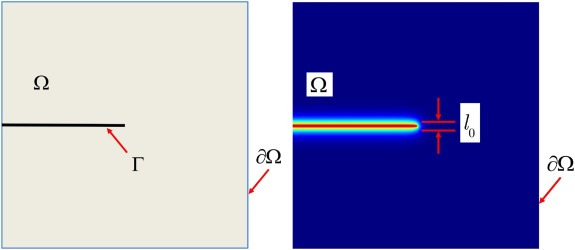
\includegraphics[width=0.5\textwidth]{figures/diffuse_edge.jpg}
\end{figure}
\end{frame}


\begin{frame}{Математическая модель}
%\vspace{-0.3cm}
\begin{block}{Уравнения динамики системы}
    \vspace{-2mm}
    \begin{gather*}
        \Div(\epsilon[\phi] \nabla \Phi) = -\rho_E \\
        \partt{\rho_E} = \Div(\sigma[\phi] \nabla \Phi) \\
        \cfrac{1}{m} \partt{\phi} = -F'_\phi( \phi; \| \nabla \Phi \|) + \cfrac{\Gamma}{2} \Delta \phi + \beta \Gamma l^2 \Div \left( \| \nabla \phi \|_2^2 \nabla \phi \right)
    \end{gather*}
    \vspace{-4mm}
\end{block}
\begin{itemize}
    \item $m$, $\Gamma$, $l$, $\beta$ -- параметры модели, константы
    \item $F(\phi; \| \nabla \Phi \|)$ -- определенная нелинейная функция
\end{itemize}
\end{frame}


\begin{frame}{Математическая модель}
\vspace{-3mm}
\begin{gather*}
    F(\phi; \| \nabla \Phi \|) = -\half \epsilon[\phi] \cdot \| \nabla \Phi \|_2^2 + \cfrac{\Gamma}{l^2} [1 - f(\phi)] \\
    \begin{alignedat}{3}
        \epsilon[\phi] &= \epsilon(\vx, t) &&= \cfrac{\epsilon_0(\vx)}{f[\phi(\vx, t)] + \delta_\epsilon} \\
        \sigma[\phi] &= \sigma(\vx, t) &&= \cfrac{\sigma_0(\vx)}{f[\phi(\vx, t)] + \delta_\sigma}
    \end{alignedat} \\[2mm]
    f(\phi) = 4 \phi^3 - 3 \phi^4
\end{gather*}
\vspace{-6mm}
\begin{itemize}
    \item $\delta_\epsilon$, $\delta_\sigma$ -- регуляризующие параметры
    \item $f(\phi)$ -- интерполирующая функция
\end{itemize}
\vspace{1mm}
\parind Модель описана в \cite{zipunova_computational} на основе \cite{pitike_dielectric_breakdown}
\end{frame}


{\nologo
\begin{frame}{Функционалы энергии}
\vspace{-5mm}
\begin{itemize}
    \item Плотность энергии электрического поля:
    \[
        w_{E} = \half \epsilon[\phi] \cdot \| \nabla \Phi \|_2^2.
    \]
    \item Плотность энергии, отнесенной к каналу пробоя:
    \[
        w_\text{br} = %
        \color{light_grey}\left[\color{black} \cfrac{\Gamma}{l^2} [1 - f(\phi)] \color{light_grey}\right]\color{black} + %
        \color{light_grey}\left[\color{black} \cfrac{\Gamma}{4} \| \nabla \phi \|_2^2 + \cfrac{\beta}{4} \Gamma l^2 \| \nabla \phi \|_2^4 \color{light_grey}\right]\color{black}.
    \]
\end{itemize}
\begin{columns}
\column{0.49\textwidth}
    \centering
    Свободная энергия Гельмгольца
    \[
        \psi = -w_E + w_\text{br}, \quad \Psi = \int\limits_\Omega \psi d \vx
    \]
\column{0.01\textwidth}
    \rule{0.4pt}{0.25\textheight}
\column{0.49\textwidth}
    \centering
    Внутренняя энергия
    \[
        w = w_E + w_\text{br}, \quad W = \int\limits_\Omega w d \vx
    \]
\end{columns}
\end{frame}
}

%!TEX root = ../main.tex

\section{Ограничения шага по времени}

{
\nologo
\begin{frame}{Разностная схема для одномерной постановки задачи}
\vspace{-2mm}
\begin{block}{Одномерная разностная задача}
	\vspace{-2mm}
	\begin{gather*}
		\cfrac{1}{m} \cfrac{\phi_j^{k + 1} - \phi_j^k}{\tau} = -F'(\phi_j^k) + \cfrac{\Gamma}{2} \cfrac{\phi_{j + 1}^k - 2 \phi_j^k + \phi_{j - 1}^k}{h^2}; \\
		\phi_j^0 = \phi_0(jh), \quad \phi_0^k = \phi_l(k \tau), \quad \phi_M^k = \phi_r(k \tau); \\
		E = \Const
	\end{gather*}
	Сетка регулярная; $\tau$ -- шаг по времени, $h$ -- шаг по пространству.
\end{block}
\vspace{-2mm}
\begin{block}{Условие устойчивости схемы}
	\[
		\tau \leqslant \cfrac{1}{m} \min \left( \cfrac{h^2}{2 \Gamma}, \cfrac{\delta^{5/3}}{3 \epsilon_0 E^2} \right).
	\]
\end{block}
\vspace{-2mm}
\begin{itemize}
	\item Получено по спектральному признаку устойчивости в окрестности $\phi = 0$ в работе \cite{ponomarev_stability}.
\end{itemize}
\end{frame}
}


\begin{frame}{Ограничения шага по времени}
\begin{itemize}
	\item Из разностной задачи с лапласианом:
\end{itemize}
\vspace{-5mm}
\begin{center}\begin{minipage}{0.4\textwidth}\begin{alertblock}{}
\[
	\tau \leqslant \cfrac{h^2}{2 \Gamma}
\]
\vspace{-3mm}
\end{alertblock}\end{minipage}\end{center}
\begin{itemize}
	\item Из вида функции деградации свойств среды:
\end{itemize}
\vspace{-5mm}
\begin{center}\begin{minipage}{0.4\textwidth}\begin{block}{}
\[
	\tau \leqslant \cfrac{\delta^{5/3}}{3 \epsilon_0 E^2}
\]
\vspace{-3mm}
\end{block}\end{minipage}\end{center}
\begin{itemize}
	\item По времени релаксации заряда в среде:
\end{itemize}
\vspace{-5mm}
\begin{center}\begin{minipage}{0.4\textwidth}\begin{alertblock}{}
\[
	\tau \ll \widetilde{\tau} = \cfrac{\epsilon[\phi]}{\sigma[\phi]}
\]
\vspace{-3mm}
\end{alertblock}\end{minipage}\end{center}
\end{frame}

%!TEX root = ../main.tex

\section{Сравнение методов адаптации}

\begin{frame}{Общий вид схемы с адаптивным шагом}
\begin{itemize}
	\item Вводится переменный шаг $\tau^k$:
	\[
		\phi_j^{k + 1} = \phi_j^k + m \tau^k \left[ -F'(\phi_j^k) + \cfrac{\Gamma}{2} \cfrac{\phi_{j + 1}^k - 2 \phi_j^k + \phi_{j - 1}^k}{h^2} \right]
	\]
	\item Значение $\tau^k$ ограничено заранее выбранными $\tau_{\min}$ и $\tau_{\max}$:
	\[
		\tau^k = \max \left[ \tau_{\min}, \min( \tau_{\max}, \widetilde{\tau}^k) \right]
	\]
\end{itemize}
\end{frame}


\begin{frame}{Методы адаптации}
\vspace{-0.7cm}
\begin{center}\begin{minipage}{0.95\textwidth}\begin{block}{Методы адаптации}
	\begin{itemize}
		\item По фазовому полю:
	\end{itemize}
	\[
		\widetilde{\tau}_1^k = \cfrac{\Tol_1}{\left\| [ \partial \phi / \partial t]_h \right\|_C}
	\]
	\begin{itemize}
		\item По полной энергии:
	\end{itemize}
	\[
		\widetilde{\tau}_2^k = \cfrac{\Tol_2}{\left| [d \Pi / dt]_h \right|}
	\]
\end{block}\end{minipage}\end{center}
Предложены в статьях \cite{li_time_step} и \cite{zhang_time_step}.
\end{frame}


{\nologo
\begin{frame}{Методы адаптации}
\vspace{-4mm}
\begin{itemize}
	\item Условие устойчивости схемы \cite{ponomarev_stability}:
	\vspace{-2mm}

	\[
		\tau \leqslant \cfrac{1}{4m} \min \left( \cfrac{h^2}{\Gamma}, \cfrac{\delta^{5/3}}{\epsilon_0 \| \nabla \Phi \|^2} \right)
	\]
	\vspace{-3mm}
	\item Неравенство со вторым аргументом $\min$ можно переписать в виде
	\vspace{-1mm}
	\[
		m \tau \max\limits_{\phi \in [0, 1]} |F''(\phi)| \leqslant 1
	\]
\end{itemize}
\vspace{-6mm}
\begin{center}\begin{minipage}{0.95\textwidth}\begin{block}{Адаптация по устойчивости}
	\[
		\widetilde{\tau}_3^k = \cfrac{\Tol_3}{m \cdot \max\limits_{j = 0}^N G(\phi_j^k)},
	\]
	где $G(\phi)$ мажорирует $|F''(\phi)|$
\end{block}\end{minipage}\end{center}
\end{frame}
}


\begin{frame}{Вычислительный эксперимент}
\vspace{-2mm}
\begin{figure}
	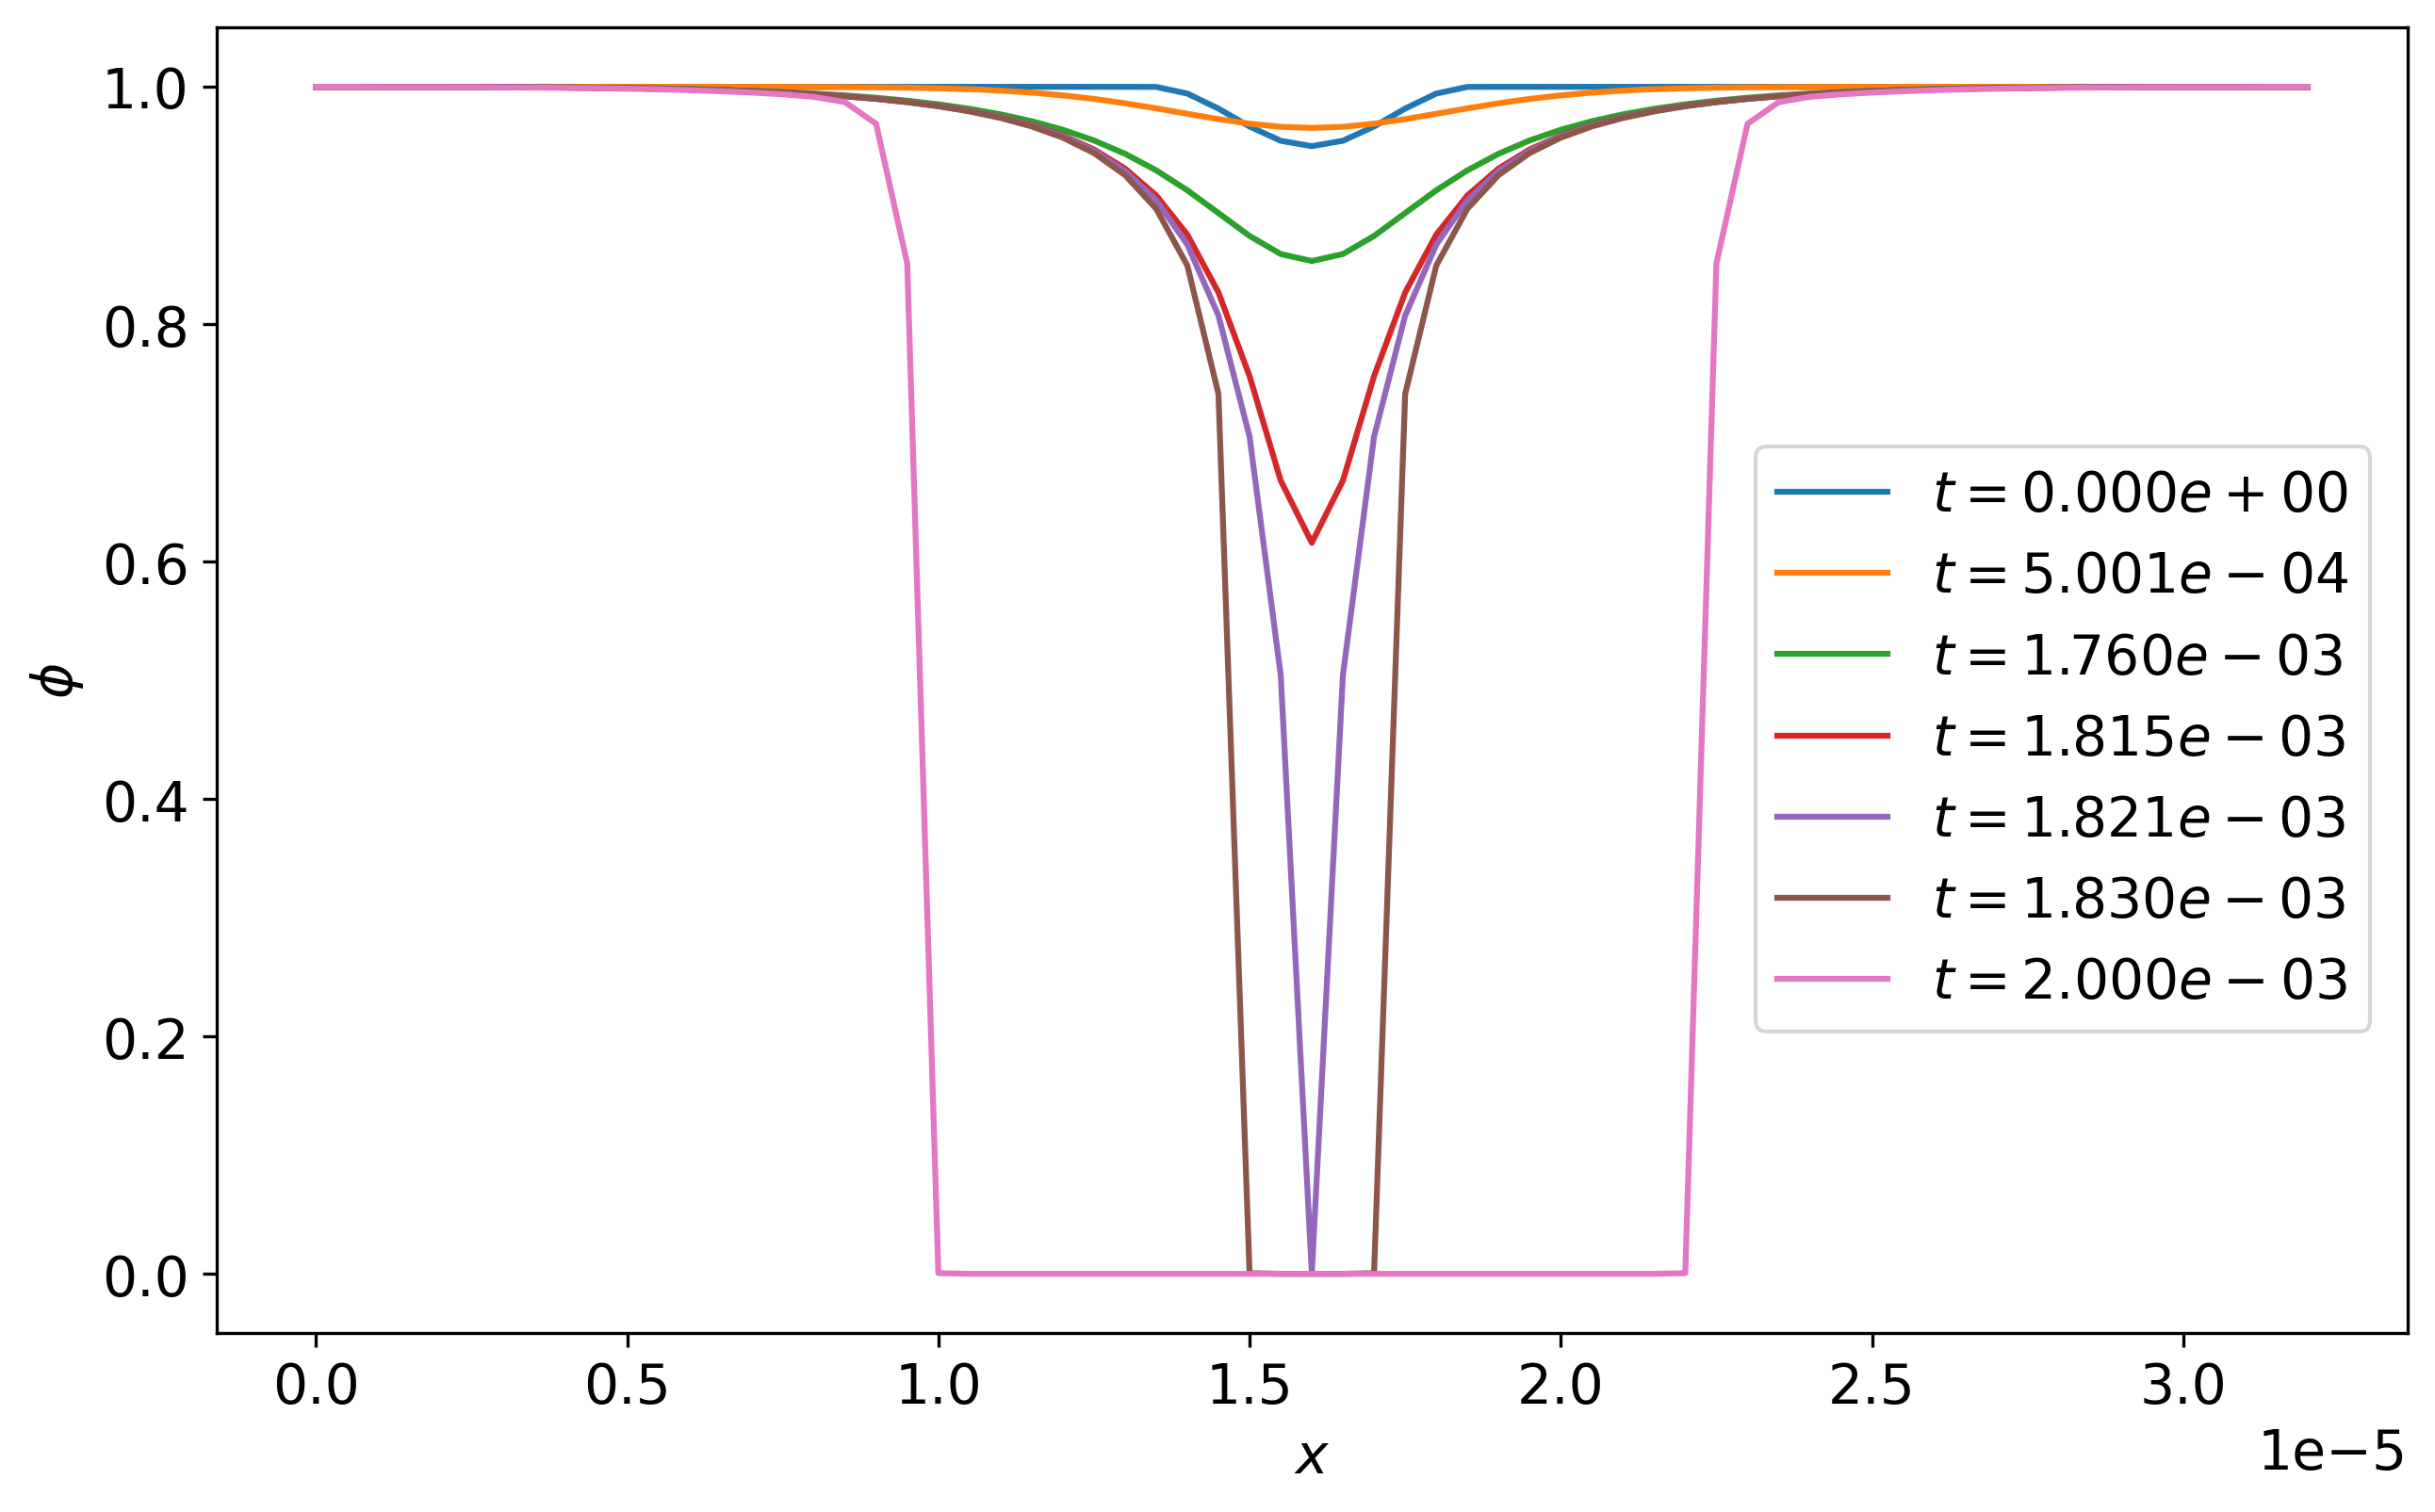
\includegraphics[width=0.81\textwidth]{figures/solution_basic.png}
\end{figure}
\end{frame}


\begin{frame}{Вычислительный эксперимент}
\vspace{-0.2cm}
\begin{center}
	Ошибка решения при ускорении
\end{center}
\vspace{-0.3cm}
\begin{figure}
	\hspace*{-0.5cm}
	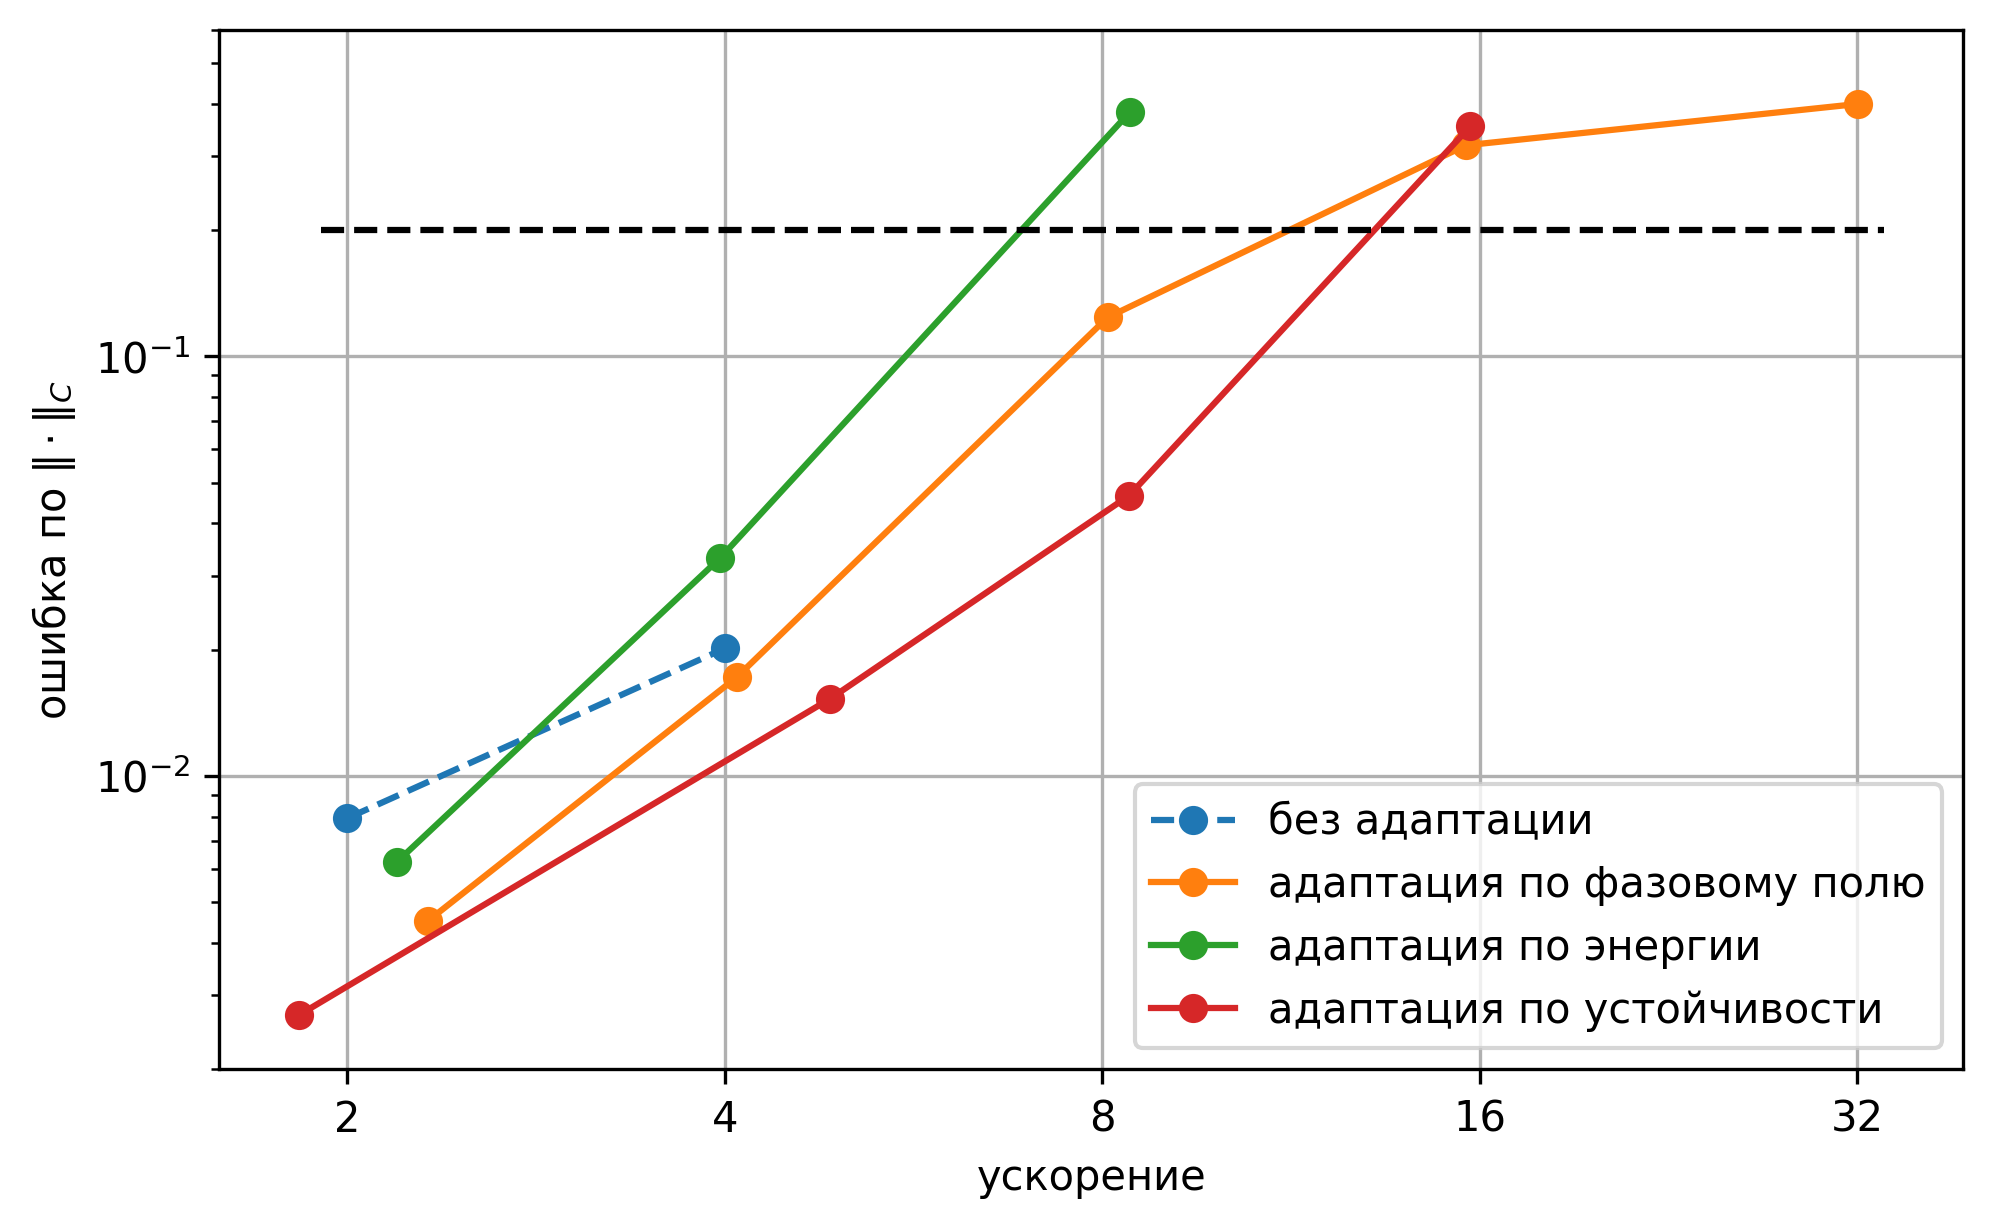
\includegraphics[width=0.75\textwidth]{figures/method_errors.png}
\end{figure}
\end{frame}


\begin{frame}{Вычислительный эксперимент}
\vspace{-0.2cm}
\begin{center}
	Ошибка решения при ускорении: задан существенный $\tau_{\max}$
\end{center}
\vspace{-0.3cm}
\begin{figure}
	\hspace*{-0.5cm}
	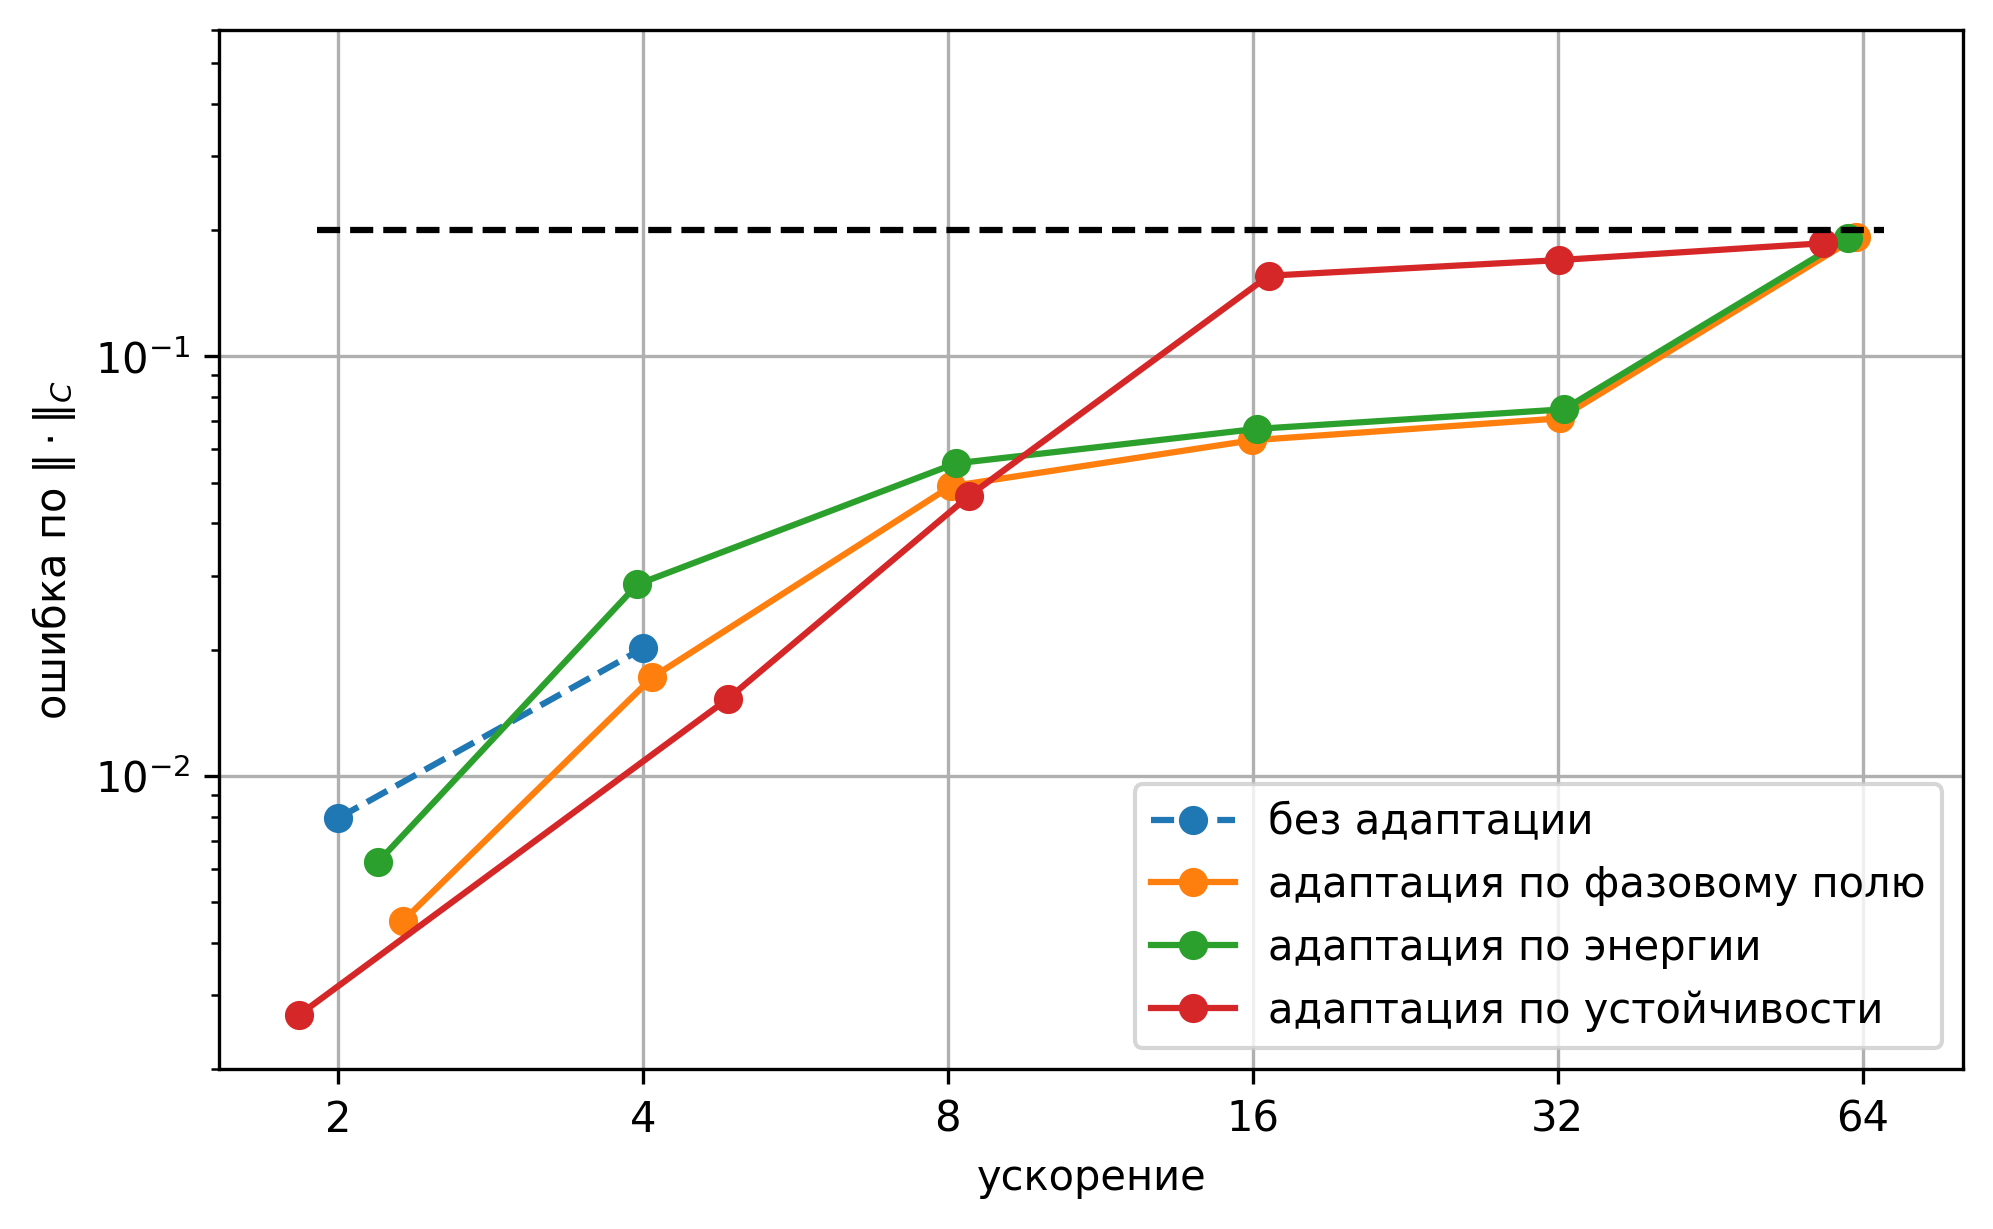
\includegraphics[width=0.75\textwidth]{figures/method_limited_errors.png}
\end{figure}
\end{frame}

%!TEX root = ../main.tex

\section{Адаптация шага в трехмерной программе}

{\nologo
\begin{frame}{Граничные условия}
\begin{columns}
\column{0.6\textwidth}
    \hfill \\[-2mm]
    \hspace*{4mm}
    \begin{tikzpicture}
        \node (image) [anchor=south west, inner sep=0pt] {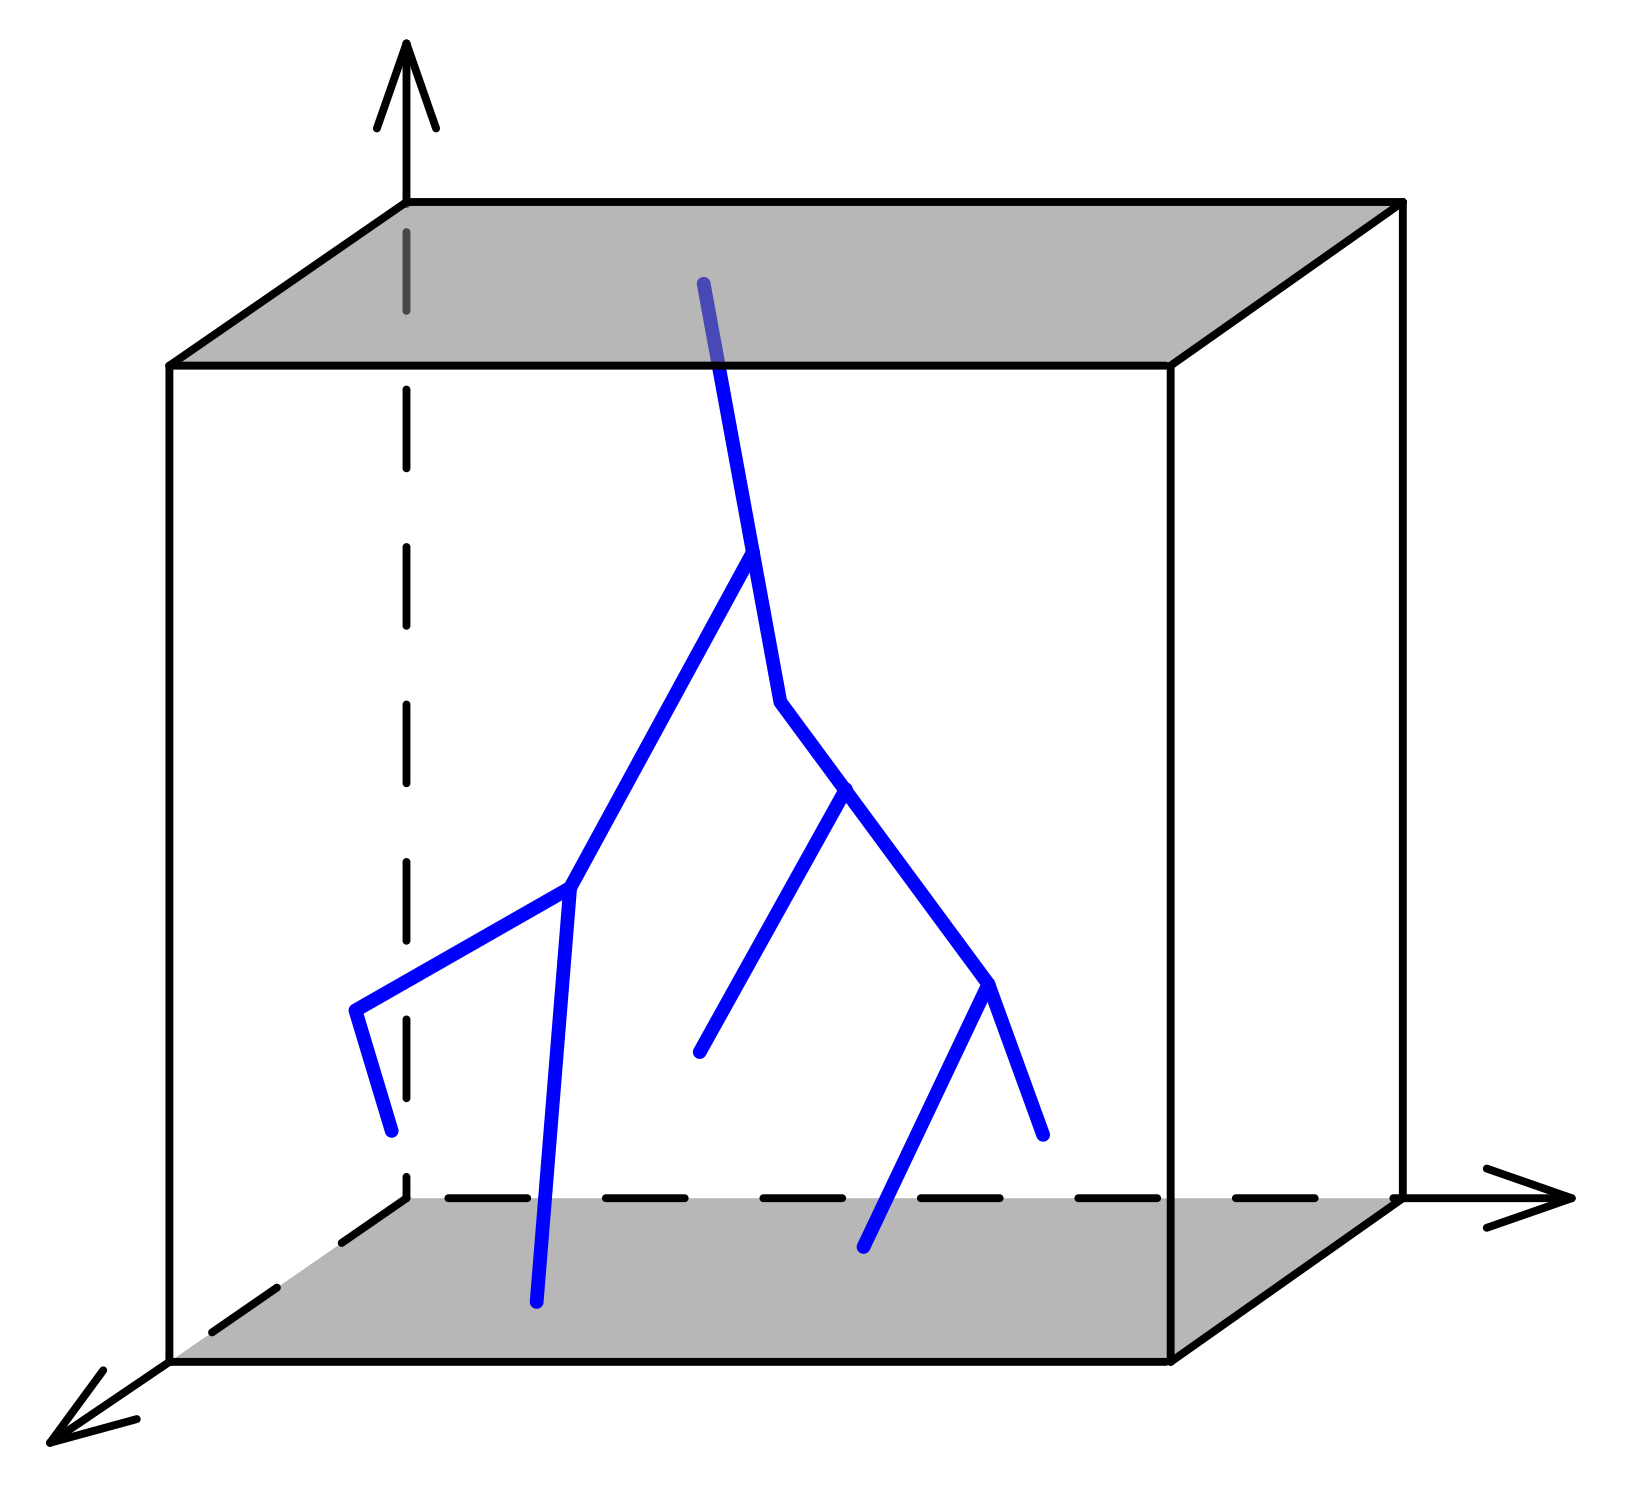
\includegraphics[scale=1.03]{figures/system_scheme.png}};
        \begin{scope}[x={(image.south east)}, y={(image.north west)}]
            \node at (.95, .15) {$x$};
            \node at (.21, .95) {$y$};
            \node at (.03, .1) {$z$};
            \node at (.523, .148) {\small $\Phi = \Phi^+(t); \quad \partvn{\phi} = 0$};
            \node at (.6, .93) {$\Phi = 0; \quad \partvn{\phi} = 0$};
            \node at (.0, .5) {$\partvn{\Phi} = 0;$};
            \node at (.015, .38) {$\phi = 1$};
        \end{scope}
    \end{tikzpicture}
\column{0.4\textwidth}
    \vspace{-5mm}
    \begin{itemize}
        \item Образец диэлектрика \\ в форме параллелепипеда:
    \end{itemize}
    \vspace{2mm}
    \[
        \clOmega = [0, L]_x \times [0, H]_y \times I_z.
    \]
    \vspace{-5mm}
    \begin{itemize}
        \item Зажат между двумя \\ проводящими пластинами \\ под напряжением.
        \item Заряды на обкладках:
    \end{itemize}
    \vspace{-4mm}
    \begin{align*}
        q^+(t) &= -\int\limits_{y = H} \epsilon \cfrac{\partial \Phi}{\partial y} dS; \\
        q^-(t) &= \int\limits_{y = 0} \epsilon \cfrac{\partial \Phi}{\partial y} dS.
    \end{align*}
\end{columns}
\end{frame}
}


\begin{frame}{Разностная схема}
\vspace{-3mm}
\begin{enumerate}
	\item $\; \Div_h \left( \epsilon[\phi] \nabla_h \hat{\Phi} \right) = - \rho_E \quad \leadsto \quad \hat{\Phi}$
	\item $\left[ \partt{\phi} \right]_h = m \cdot \left( -F'( \phi; \| \nabla_h \hat{\Phi} \|) + \cfrac{\Gamma}{2} \Delta_h \phi + \beta \Gamma l^2 \Div_h \left( \| \nabla_h \phi \|_2^2 \nabla_h \phi \right) \right)$
	\item $\left[ \partt{\rho} \right]_h = \Div_h \left( \sigma[\phi] \nabla_h \hat{\Phi} \right)$
	\item $\hat{\phi} = \phi + \tau \cdot \left[ \partt{\phi} \right]_h; \qquad \hat{\rho}_E = \rho_E + \tau \cdot \left[ \partt{\rho} \right]_h$
\end{enumerate}
\vspace{2mm}
\parind $\Pi = \sum h^3 \cdot \left( F(\phi; \| \nabla_h \Phi \|) + \cfrac{\Gamma}{4} \| \nabla_h \phi \|_2^2 + \cfrac{\beta}{4} \Gamma l^2 \| \nabla_h \phi \|_2^4 \right)$
\end{frame}


\begin{frame}{Проблемы}
\large
\begin{itemize}
	\setlength\itemsep{3mm}
	\item Нелинейная модель
	\item Сложная динамика с различным временным масштабом процессов
	\item Необходимость решать СЛАУ на каждом шаге
	\item Значительные ограничения на шаг по времени из-за параболичности оператора и нелинейности
\end{itemize}
\end{frame}


\begin{frame}{Адаптация по фазовому полю}
Работа \cite{ponomarev_adaptation}
\vspace{1mm}
\begin{block}{Формула расчета адаптивного шага}
	\[
		\tau^k = \max \left[ \taumin, \min \left( \taumax, \cfrac{\Tol}{\left\| [\partflt{\phi}]_h \right\|_C} \right) \right]
	\]
\end{block}
\vspace{1mm}
\parind Идея метода:
\[
	\| \hat{\phi} - \phi \|_C = \tau^k \cdot \left\| \left[ \partt{\phi} \right]_h \right\|_C = \cfrac{\Tol}{\left\| [\partflt{\phi}]_h \right\|_C} \cdot \left\| \left[ \partt{\phi} \right]_h \right\|_C \approx \Tol
\]
\parind Предложен в статье \cite{li_time_step}
\end{frame}


\begin{frame}{Расчет №1: <<иголка>>}
\vspace{-5mm}
\begin{figure}
	\subfloat[Начальное условие]{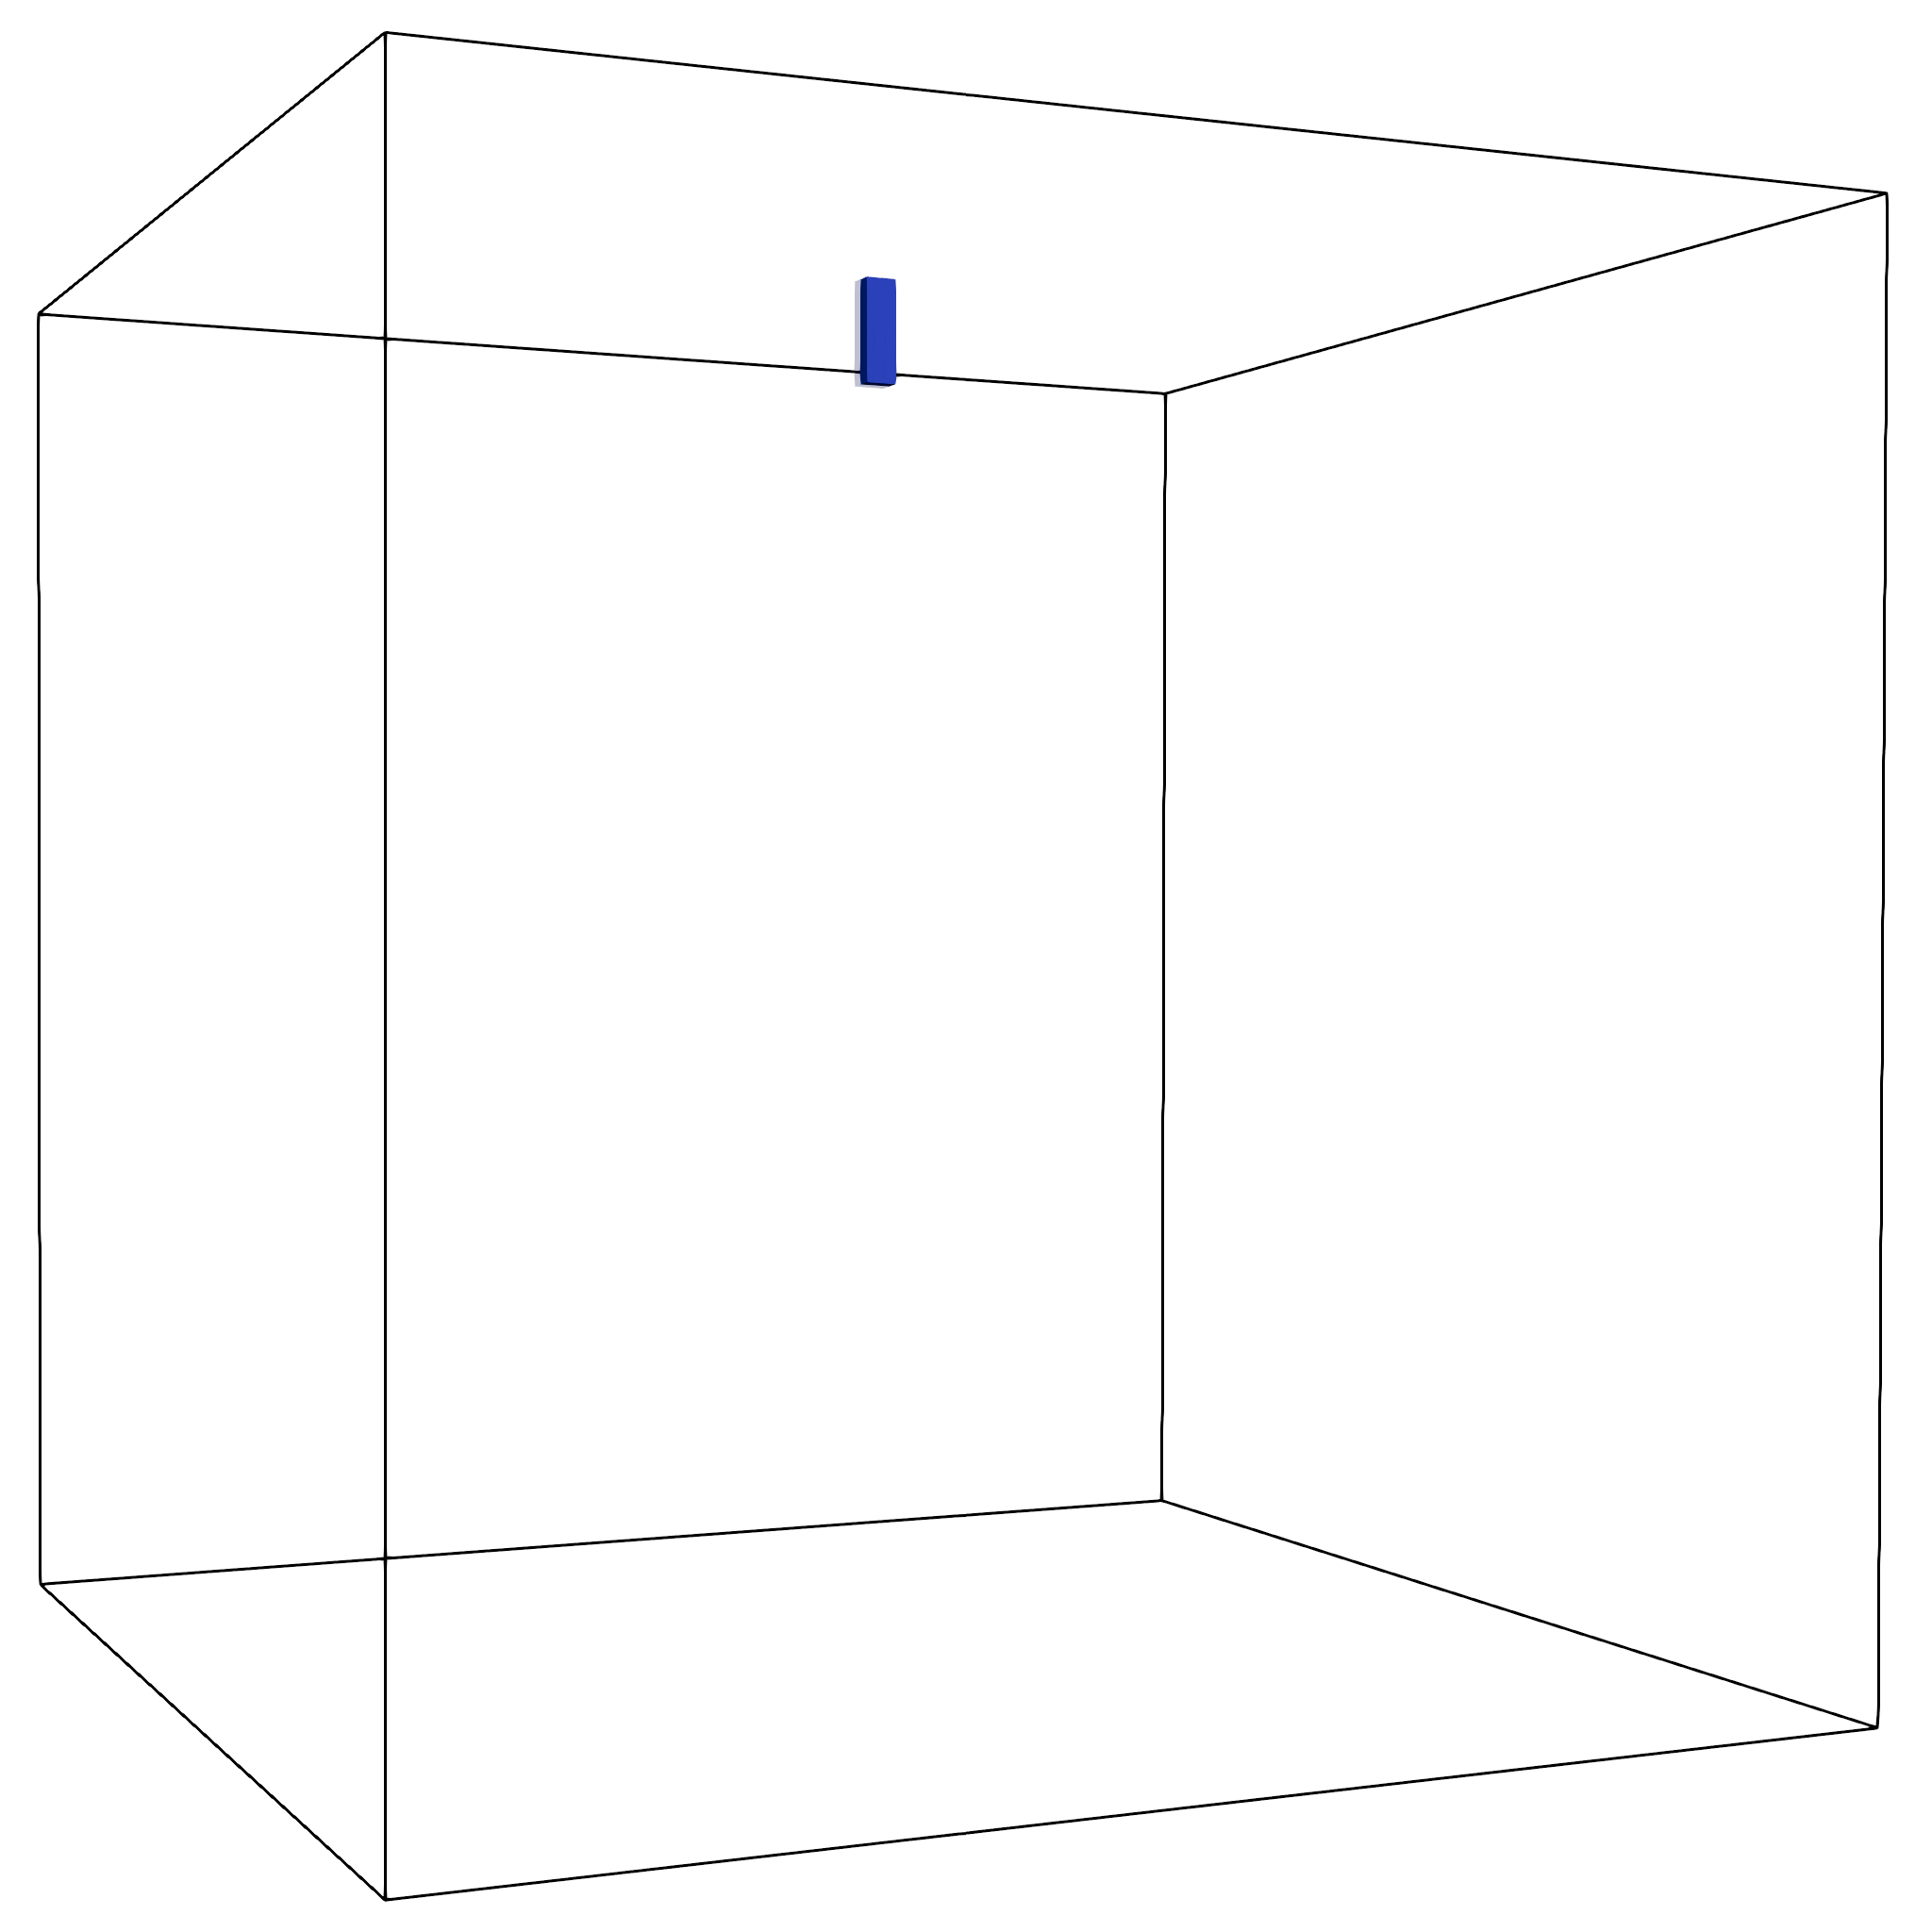
\includegraphics[width=0.333\textwidth]{figures/needle_result_1.png}}
	\subfloat[Рост канала]{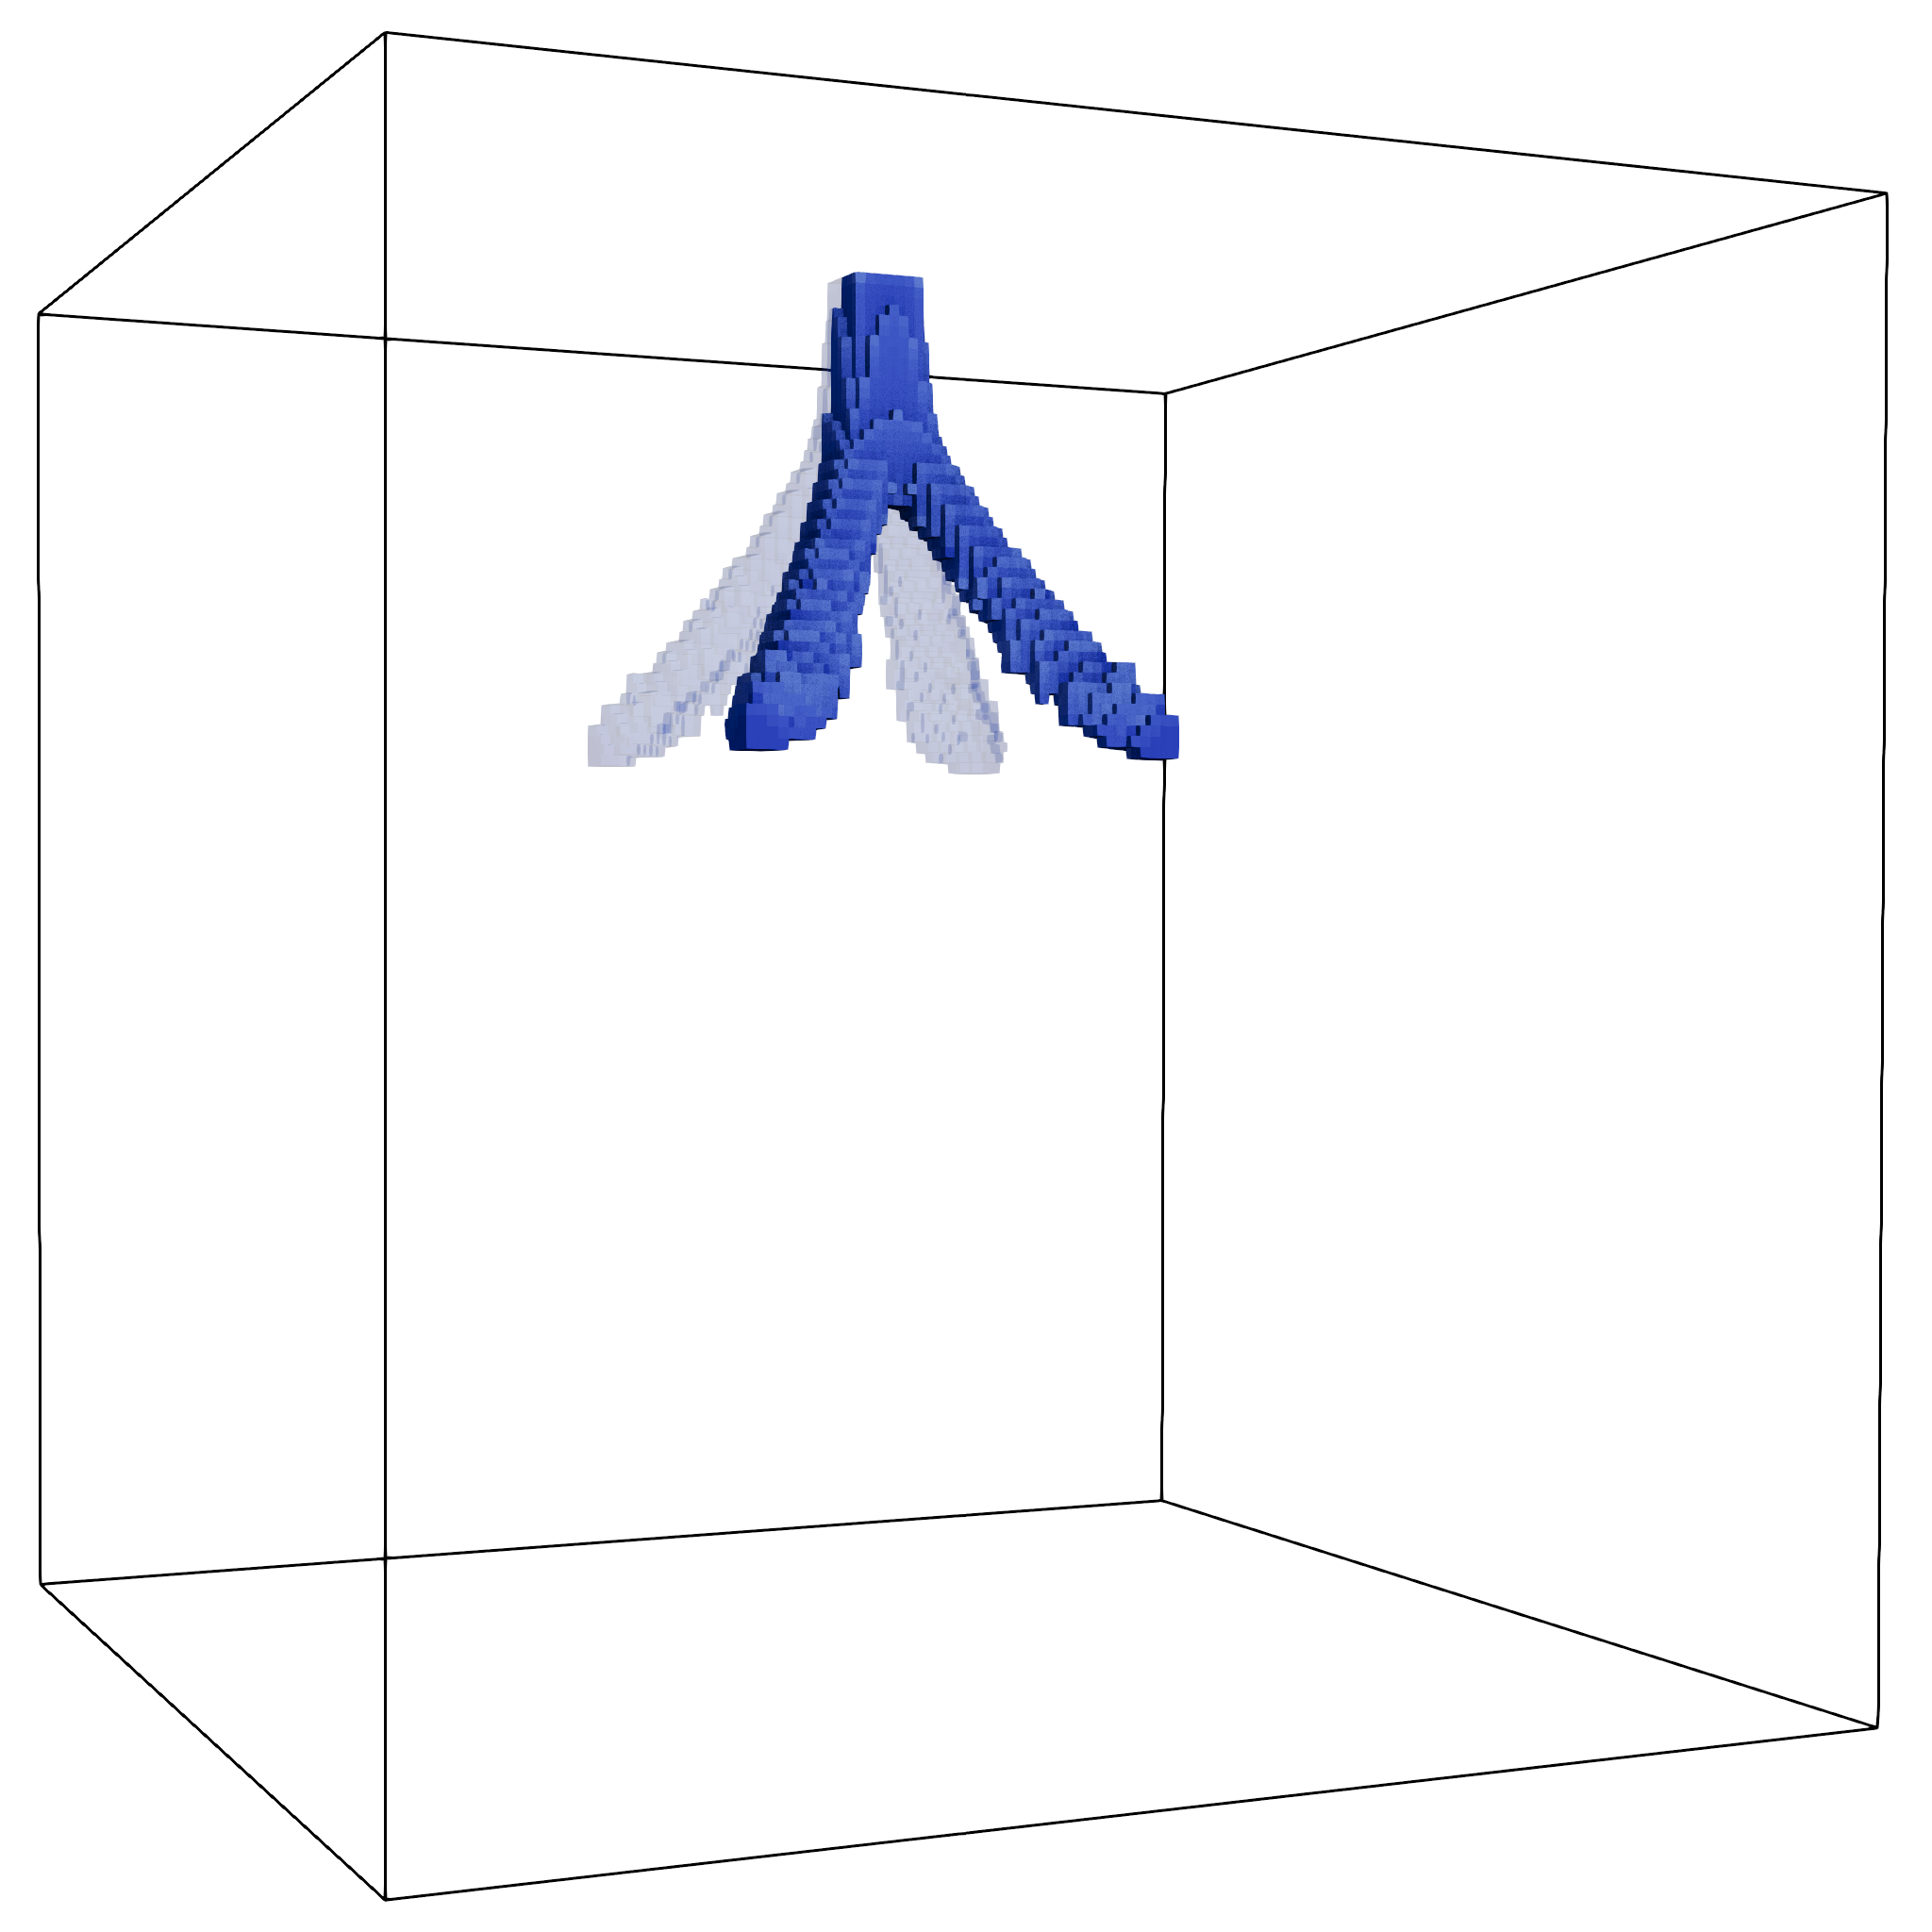
\includegraphics[width=0.333\textwidth]{figures/needle_result_2.png}}
	\subfloat[Перед пробоем <<насквозь>>]{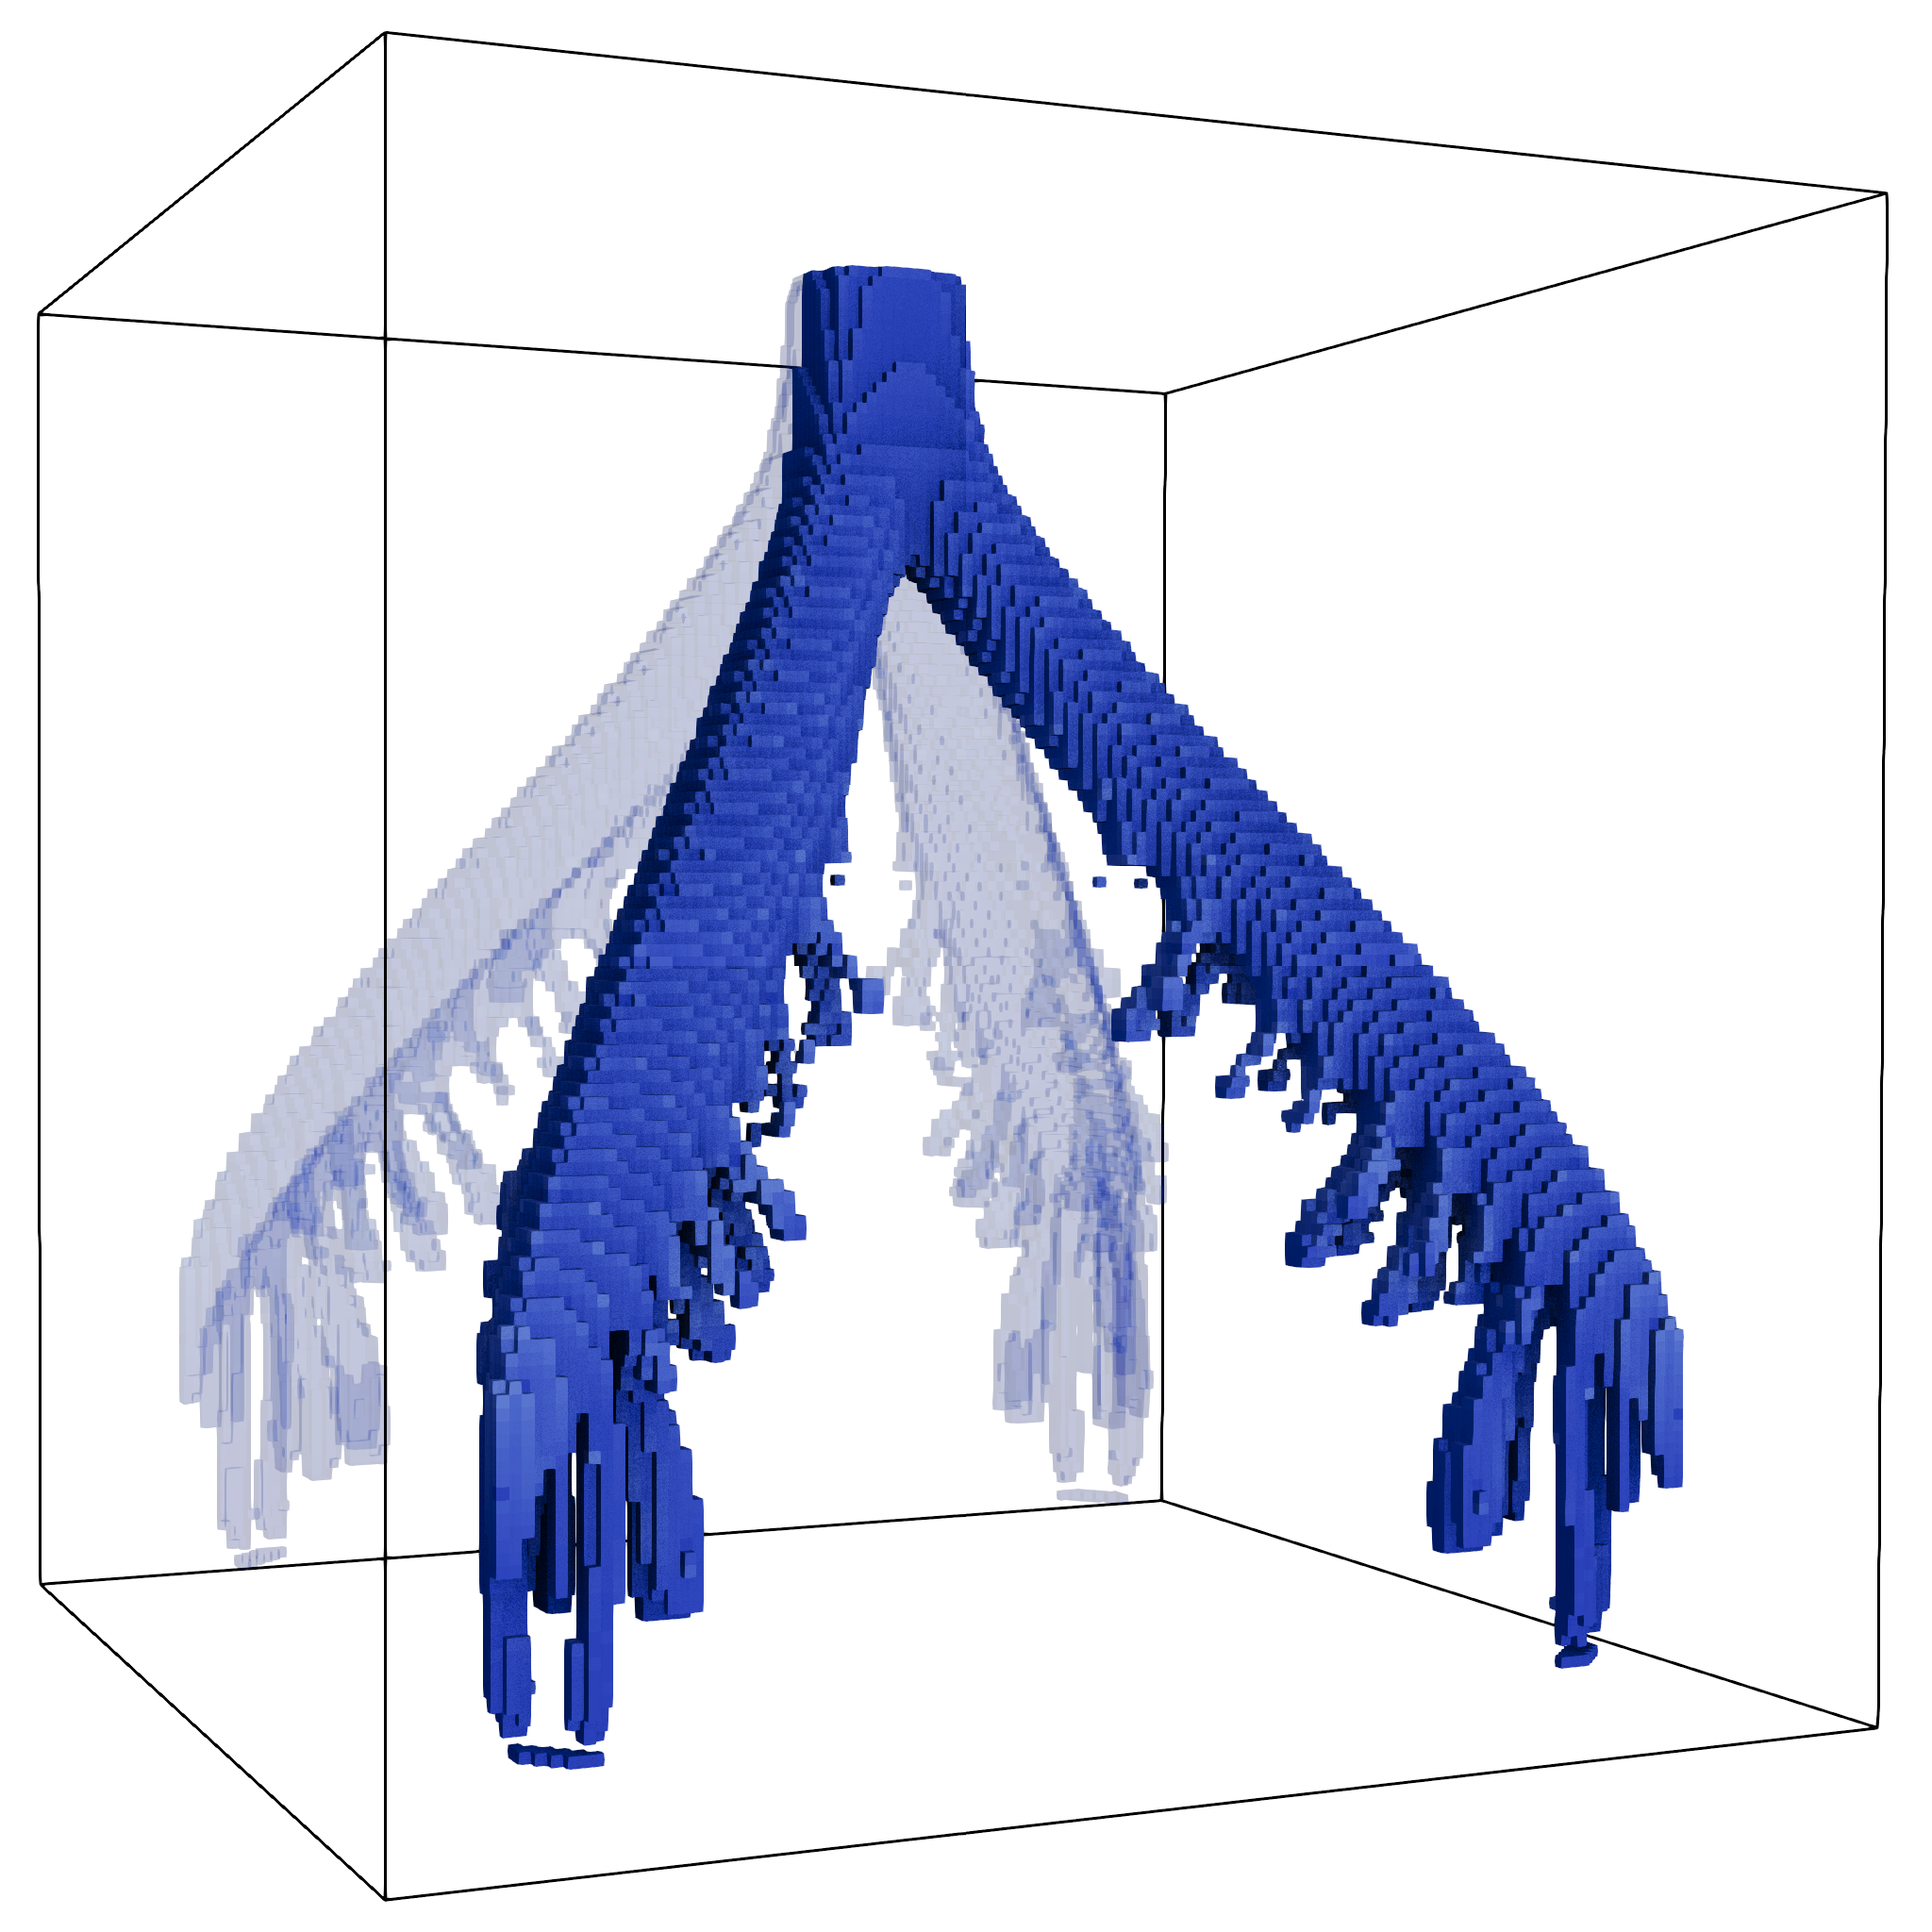
\includegraphics[width=0.333\textwidth]{figures/needle_result_3.png}}
\end{figure}
\vspace{-7mm}
\begin{minipage}[l]{0.93\textwidth}
\begin{align*}
	N_h &= 129 & T &\approx 7 \cdot 10^{-7} & \taumin &= 10^{-12} & 56 \text{ MPI-процессов} \\
	N_t &= 51000 & \Tol &= 10^{-2} & \taumax &= 10^{-7} &
\end{align*}
\end{minipage}
\end{frame}


\begin{frame}{Расчет №1: <<иголка>>}
\vspace{-4mm}
\begin{figure}
	\captionsetup[subfigure]{labelformat=empty}
	\subfloat[]{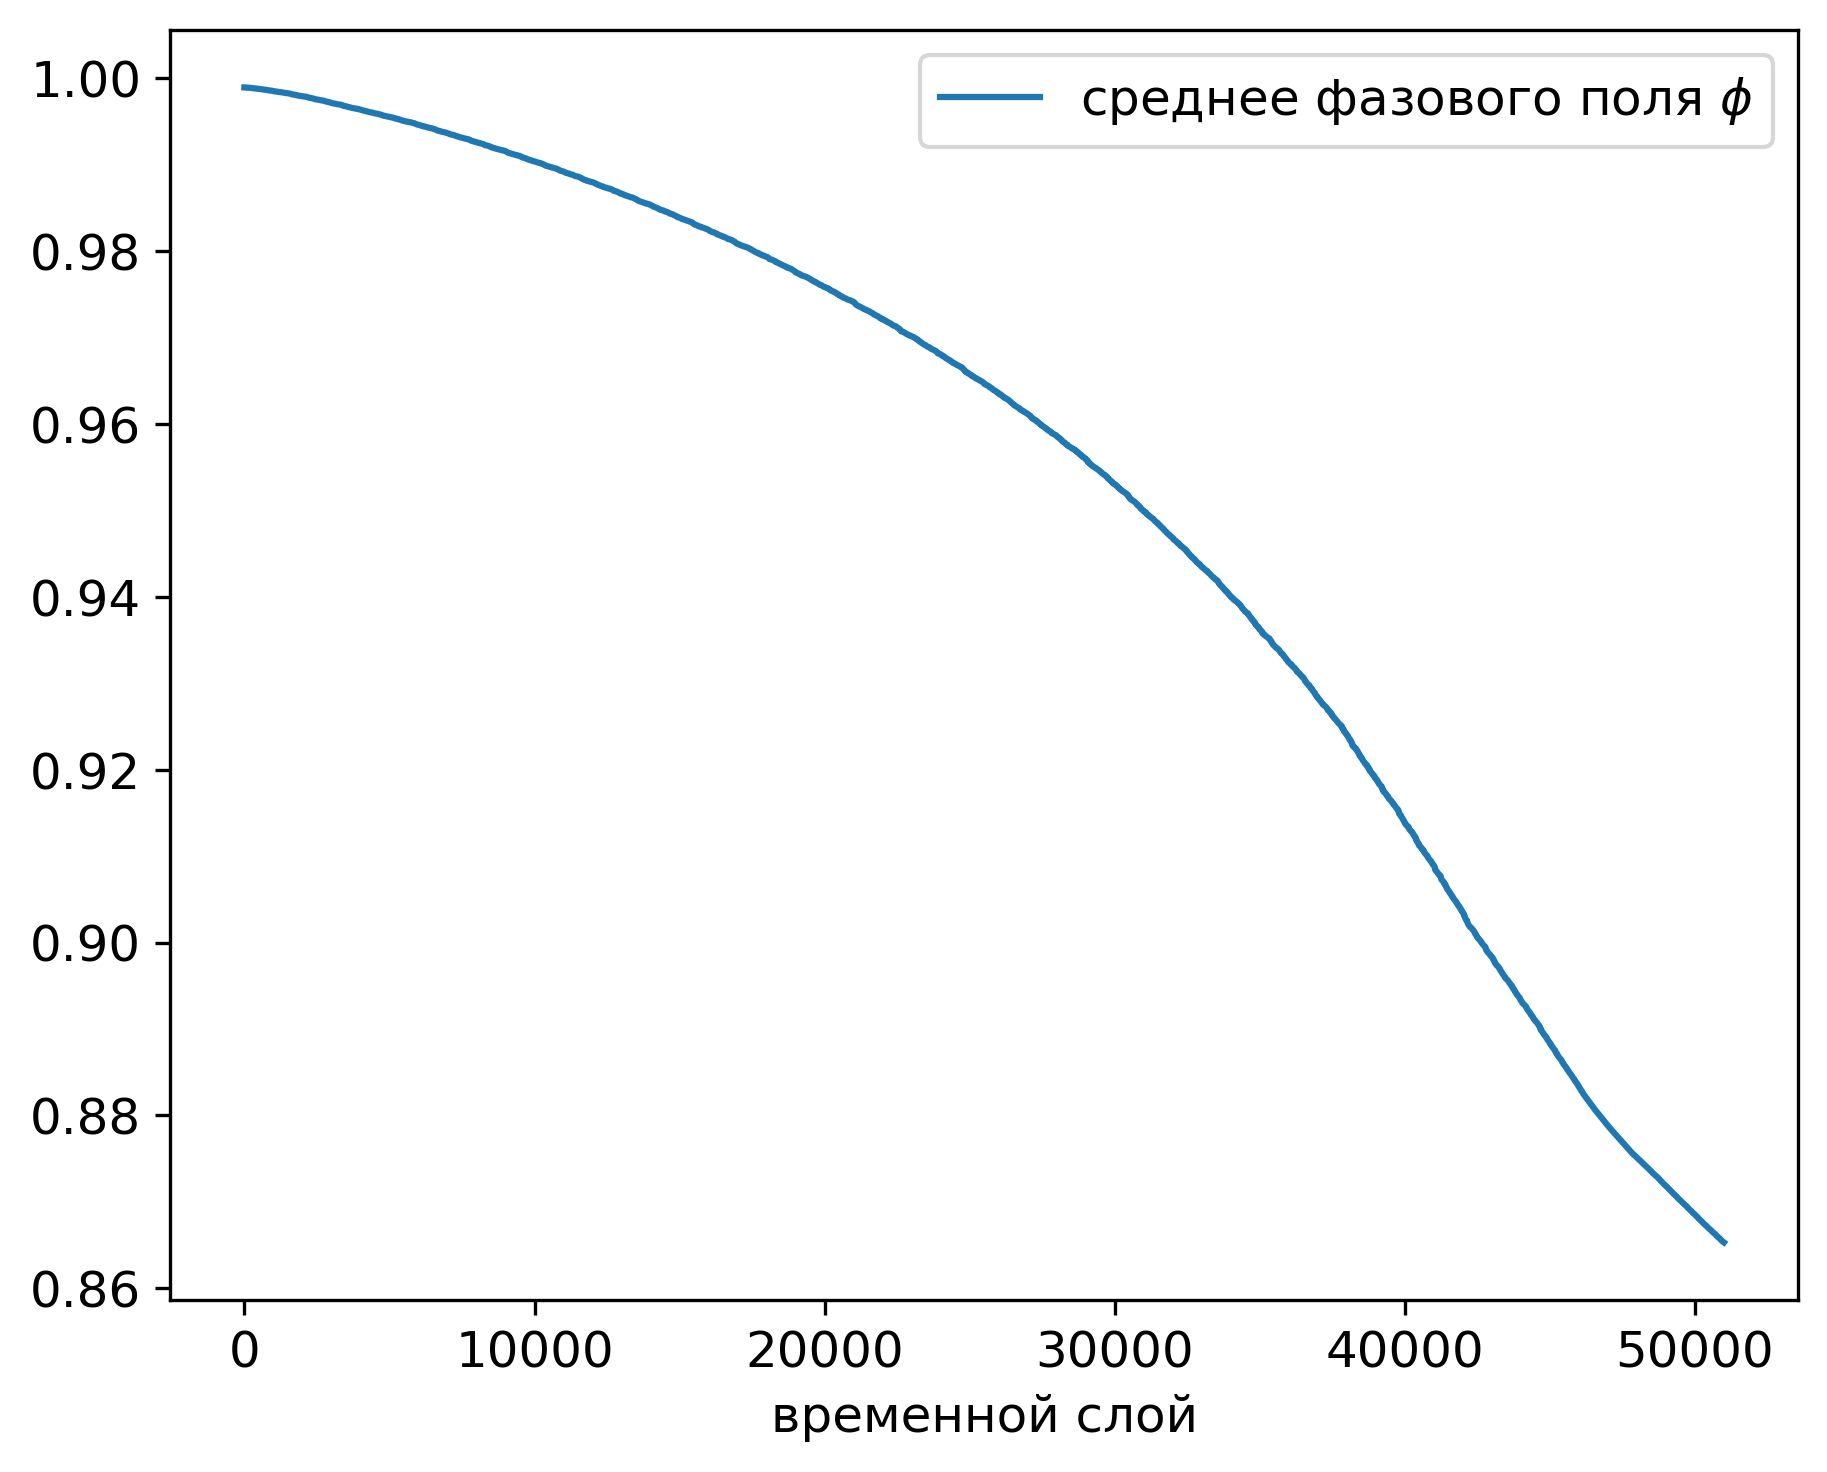
\includegraphics[width=0.49\textwidth]{figures/needle_phi_mean.png}}
	\hfill
	\subfloat[]{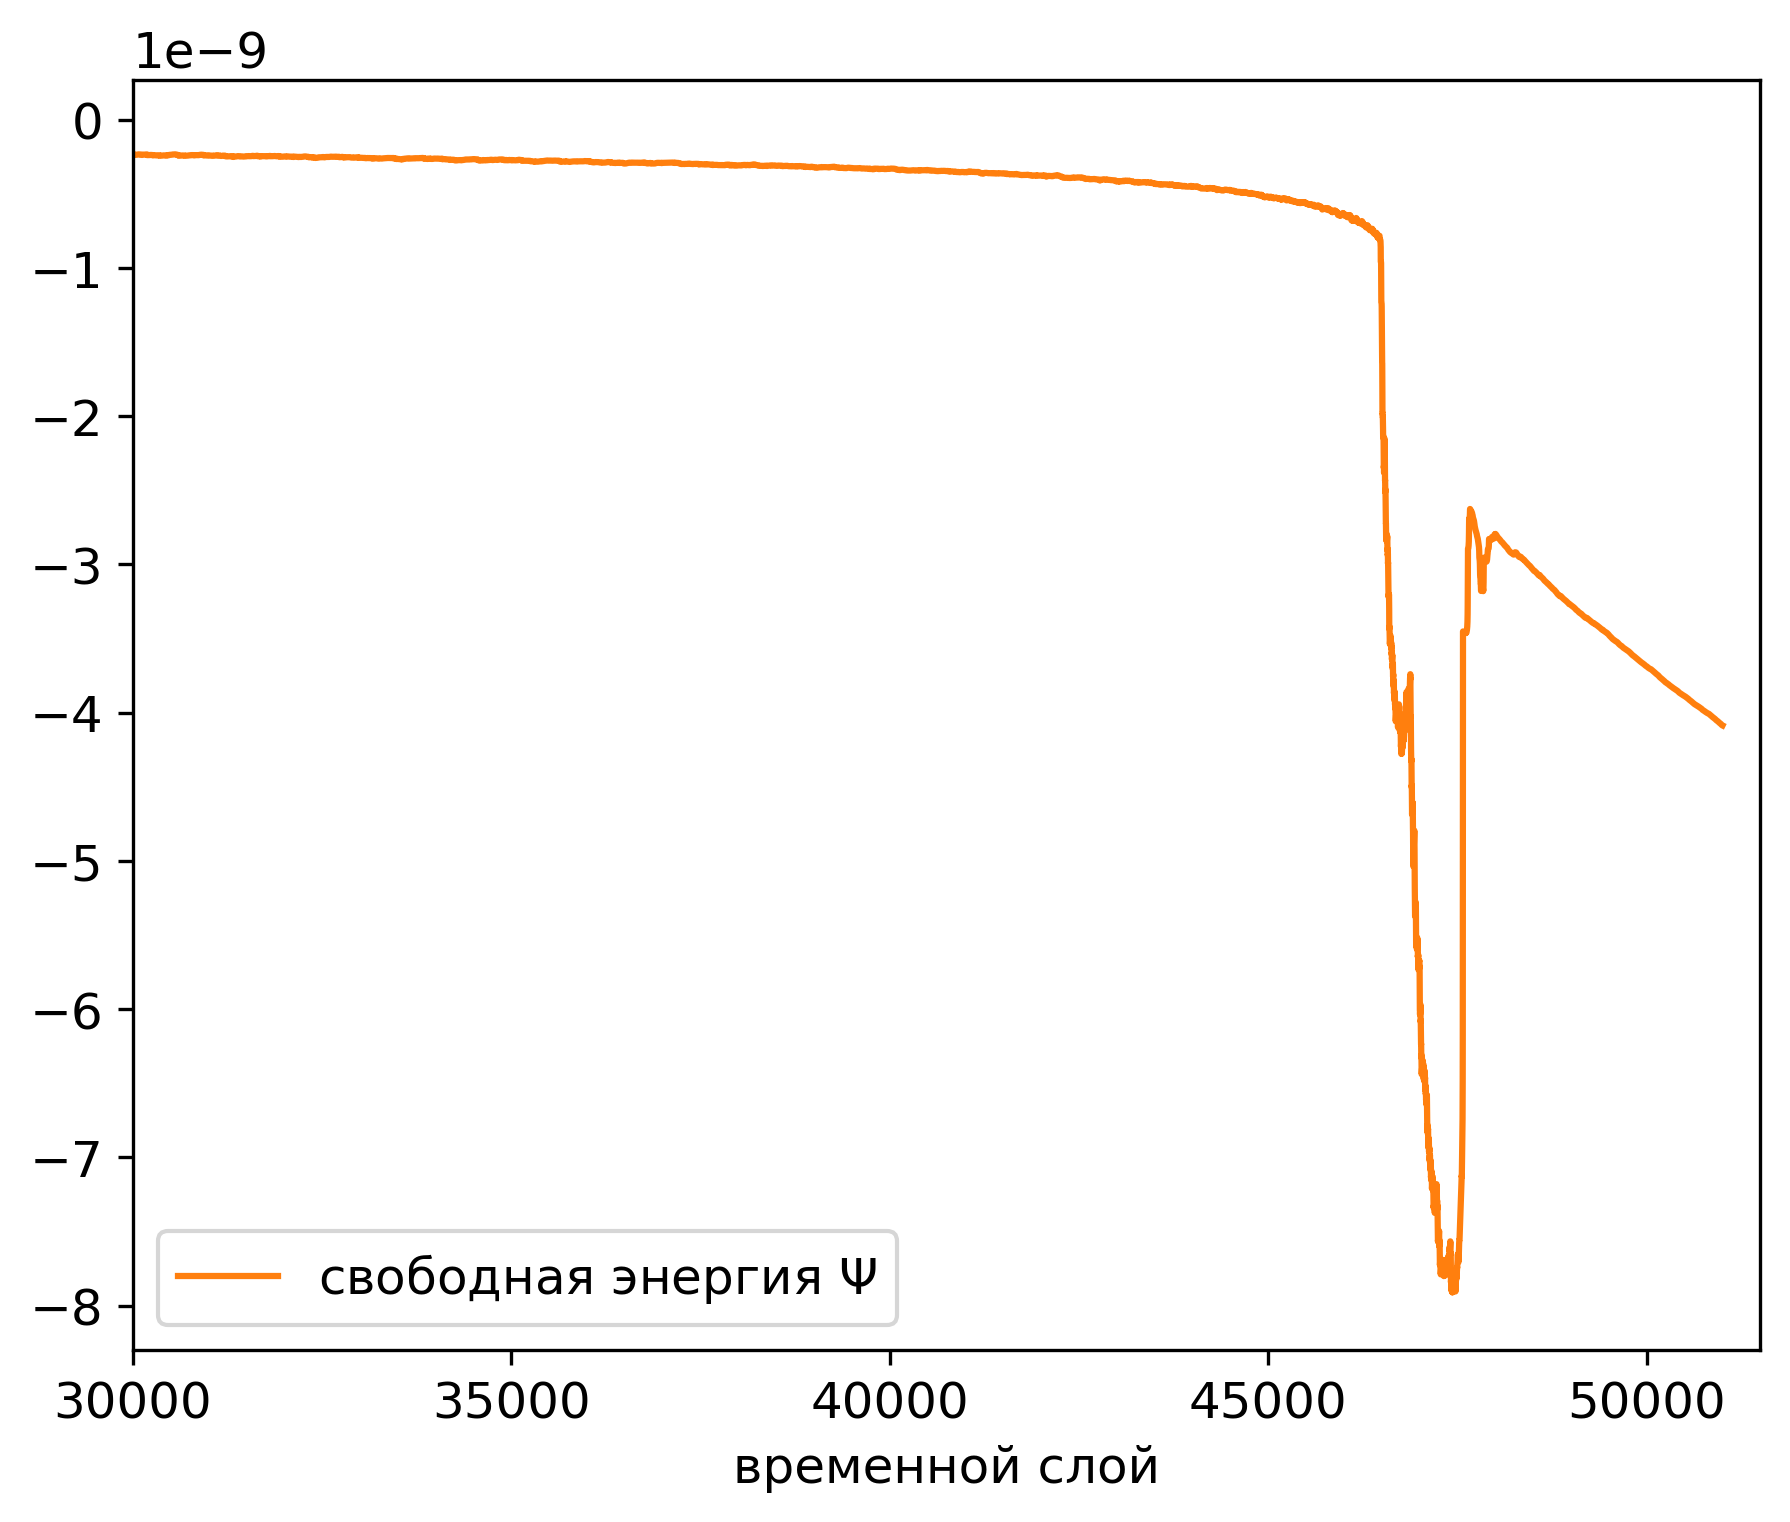
\includegraphics[width=0.49\textwidth]{figures/needle_energy.png}}
\end{figure}
\vspace{-13mm}
\begin{itemize}
    \item $\cfrac{d \Psi}{dt} = -\cfrac{1}{m} \, \intOmega (\partial \phi / \partial t)^2 d \vx \leqslant 0 \quad$ (нарушено!)
\end{itemize}
\end{frame}


\begin{frame}{Расчет №2: случайные возмущения}
\vspace{-5mm}
\begin{figure}
	\subfloat[Зародыши каналов]{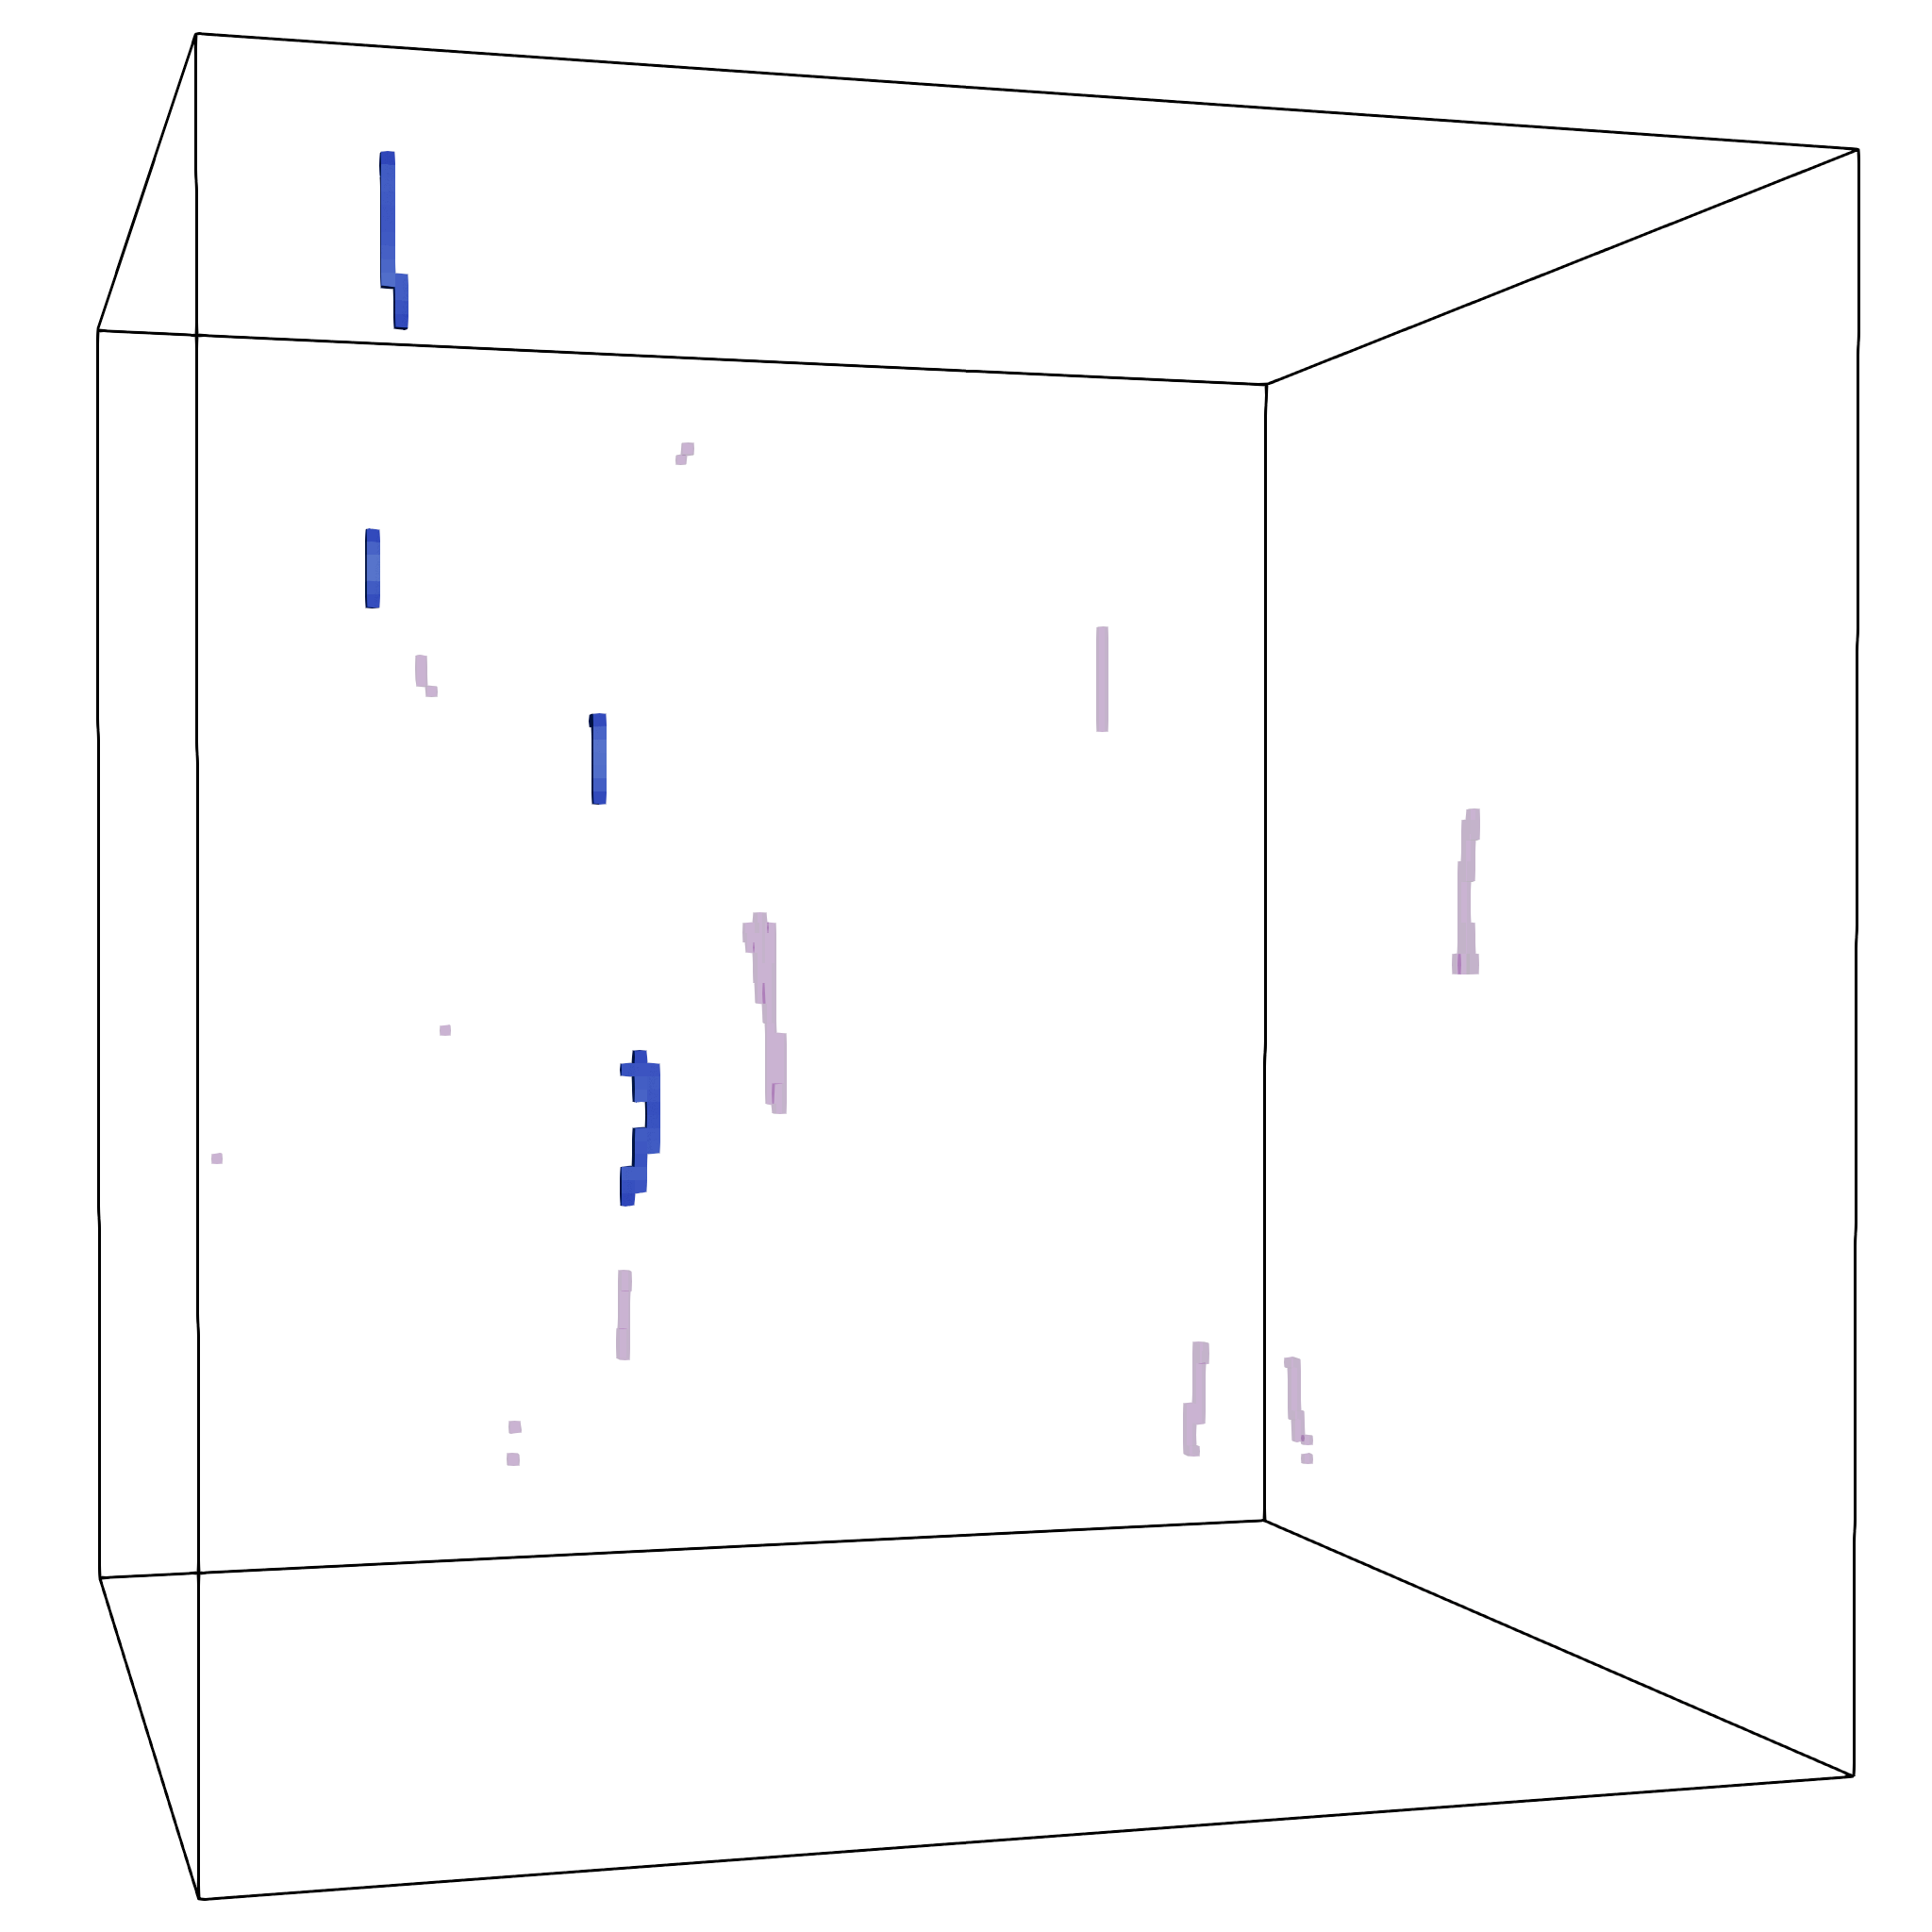
\includegraphics[width=0.333\textwidth]{figures/disturbance_result_1.png}}
	\subfloat[Рост и слияние]{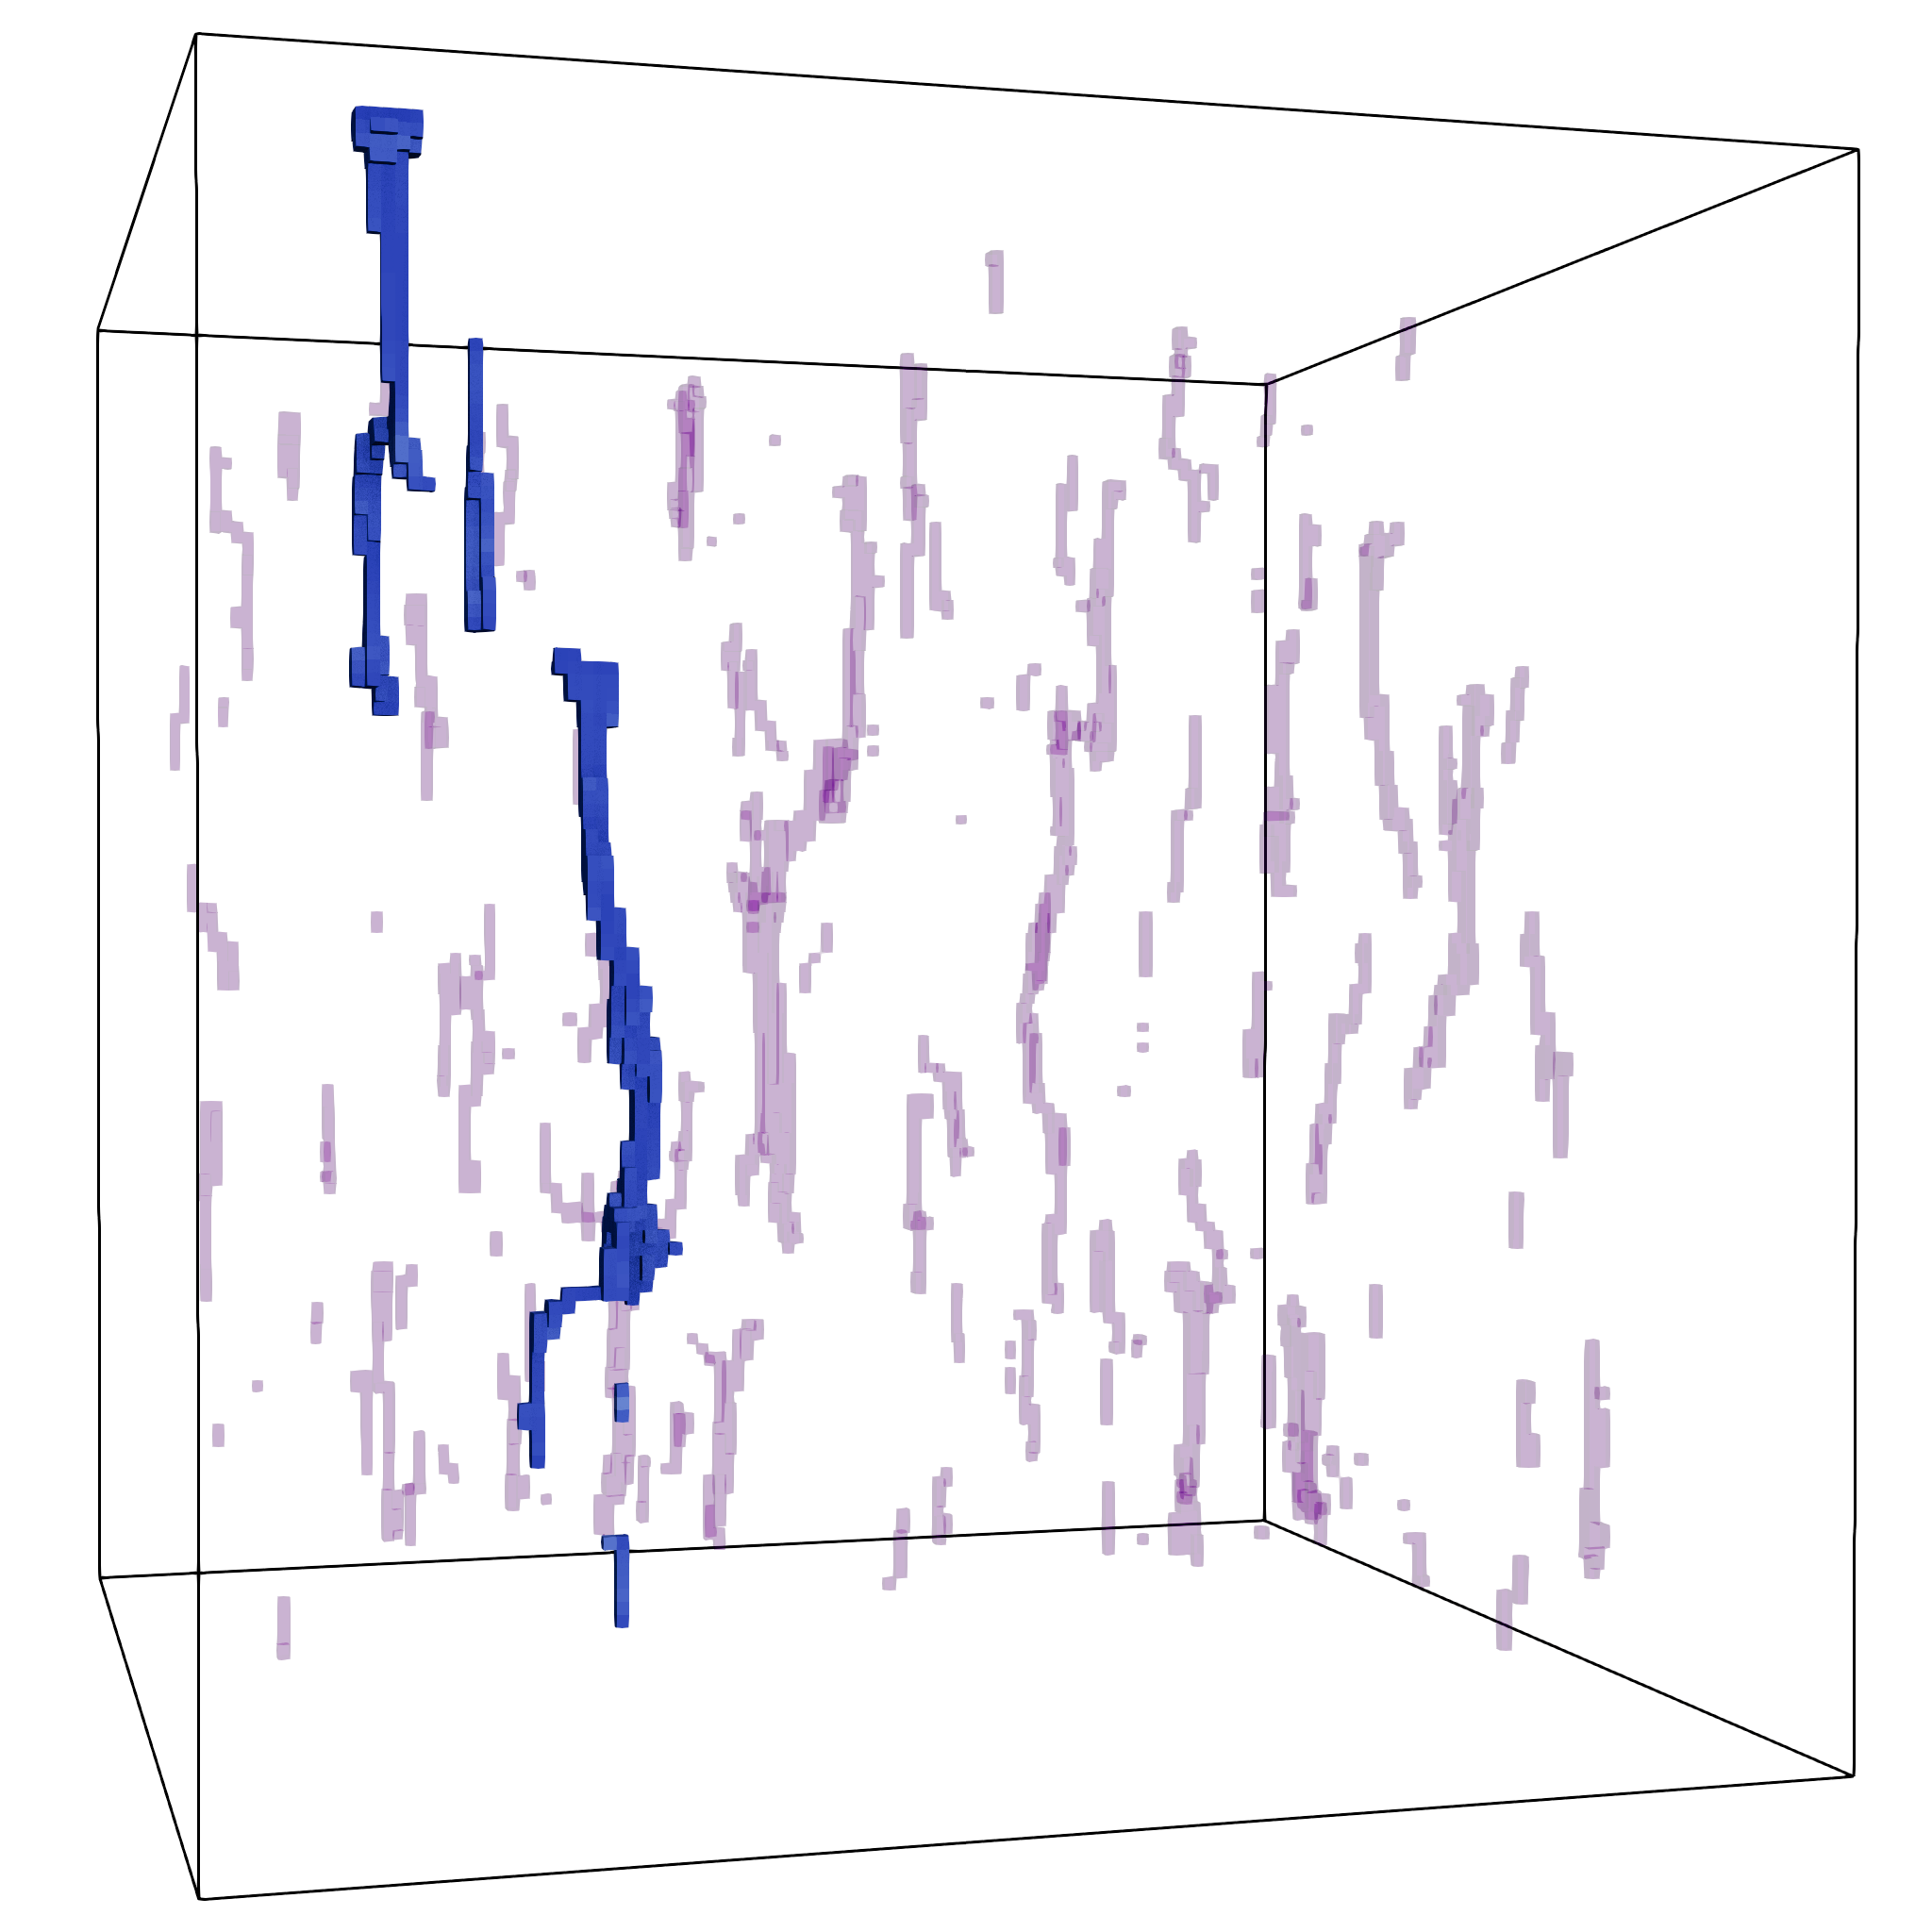
\includegraphics[width=0.333\textwidth]{figures/disturbance_result_2.png}}
	\subfloat[Пробой <<насквозь>>]{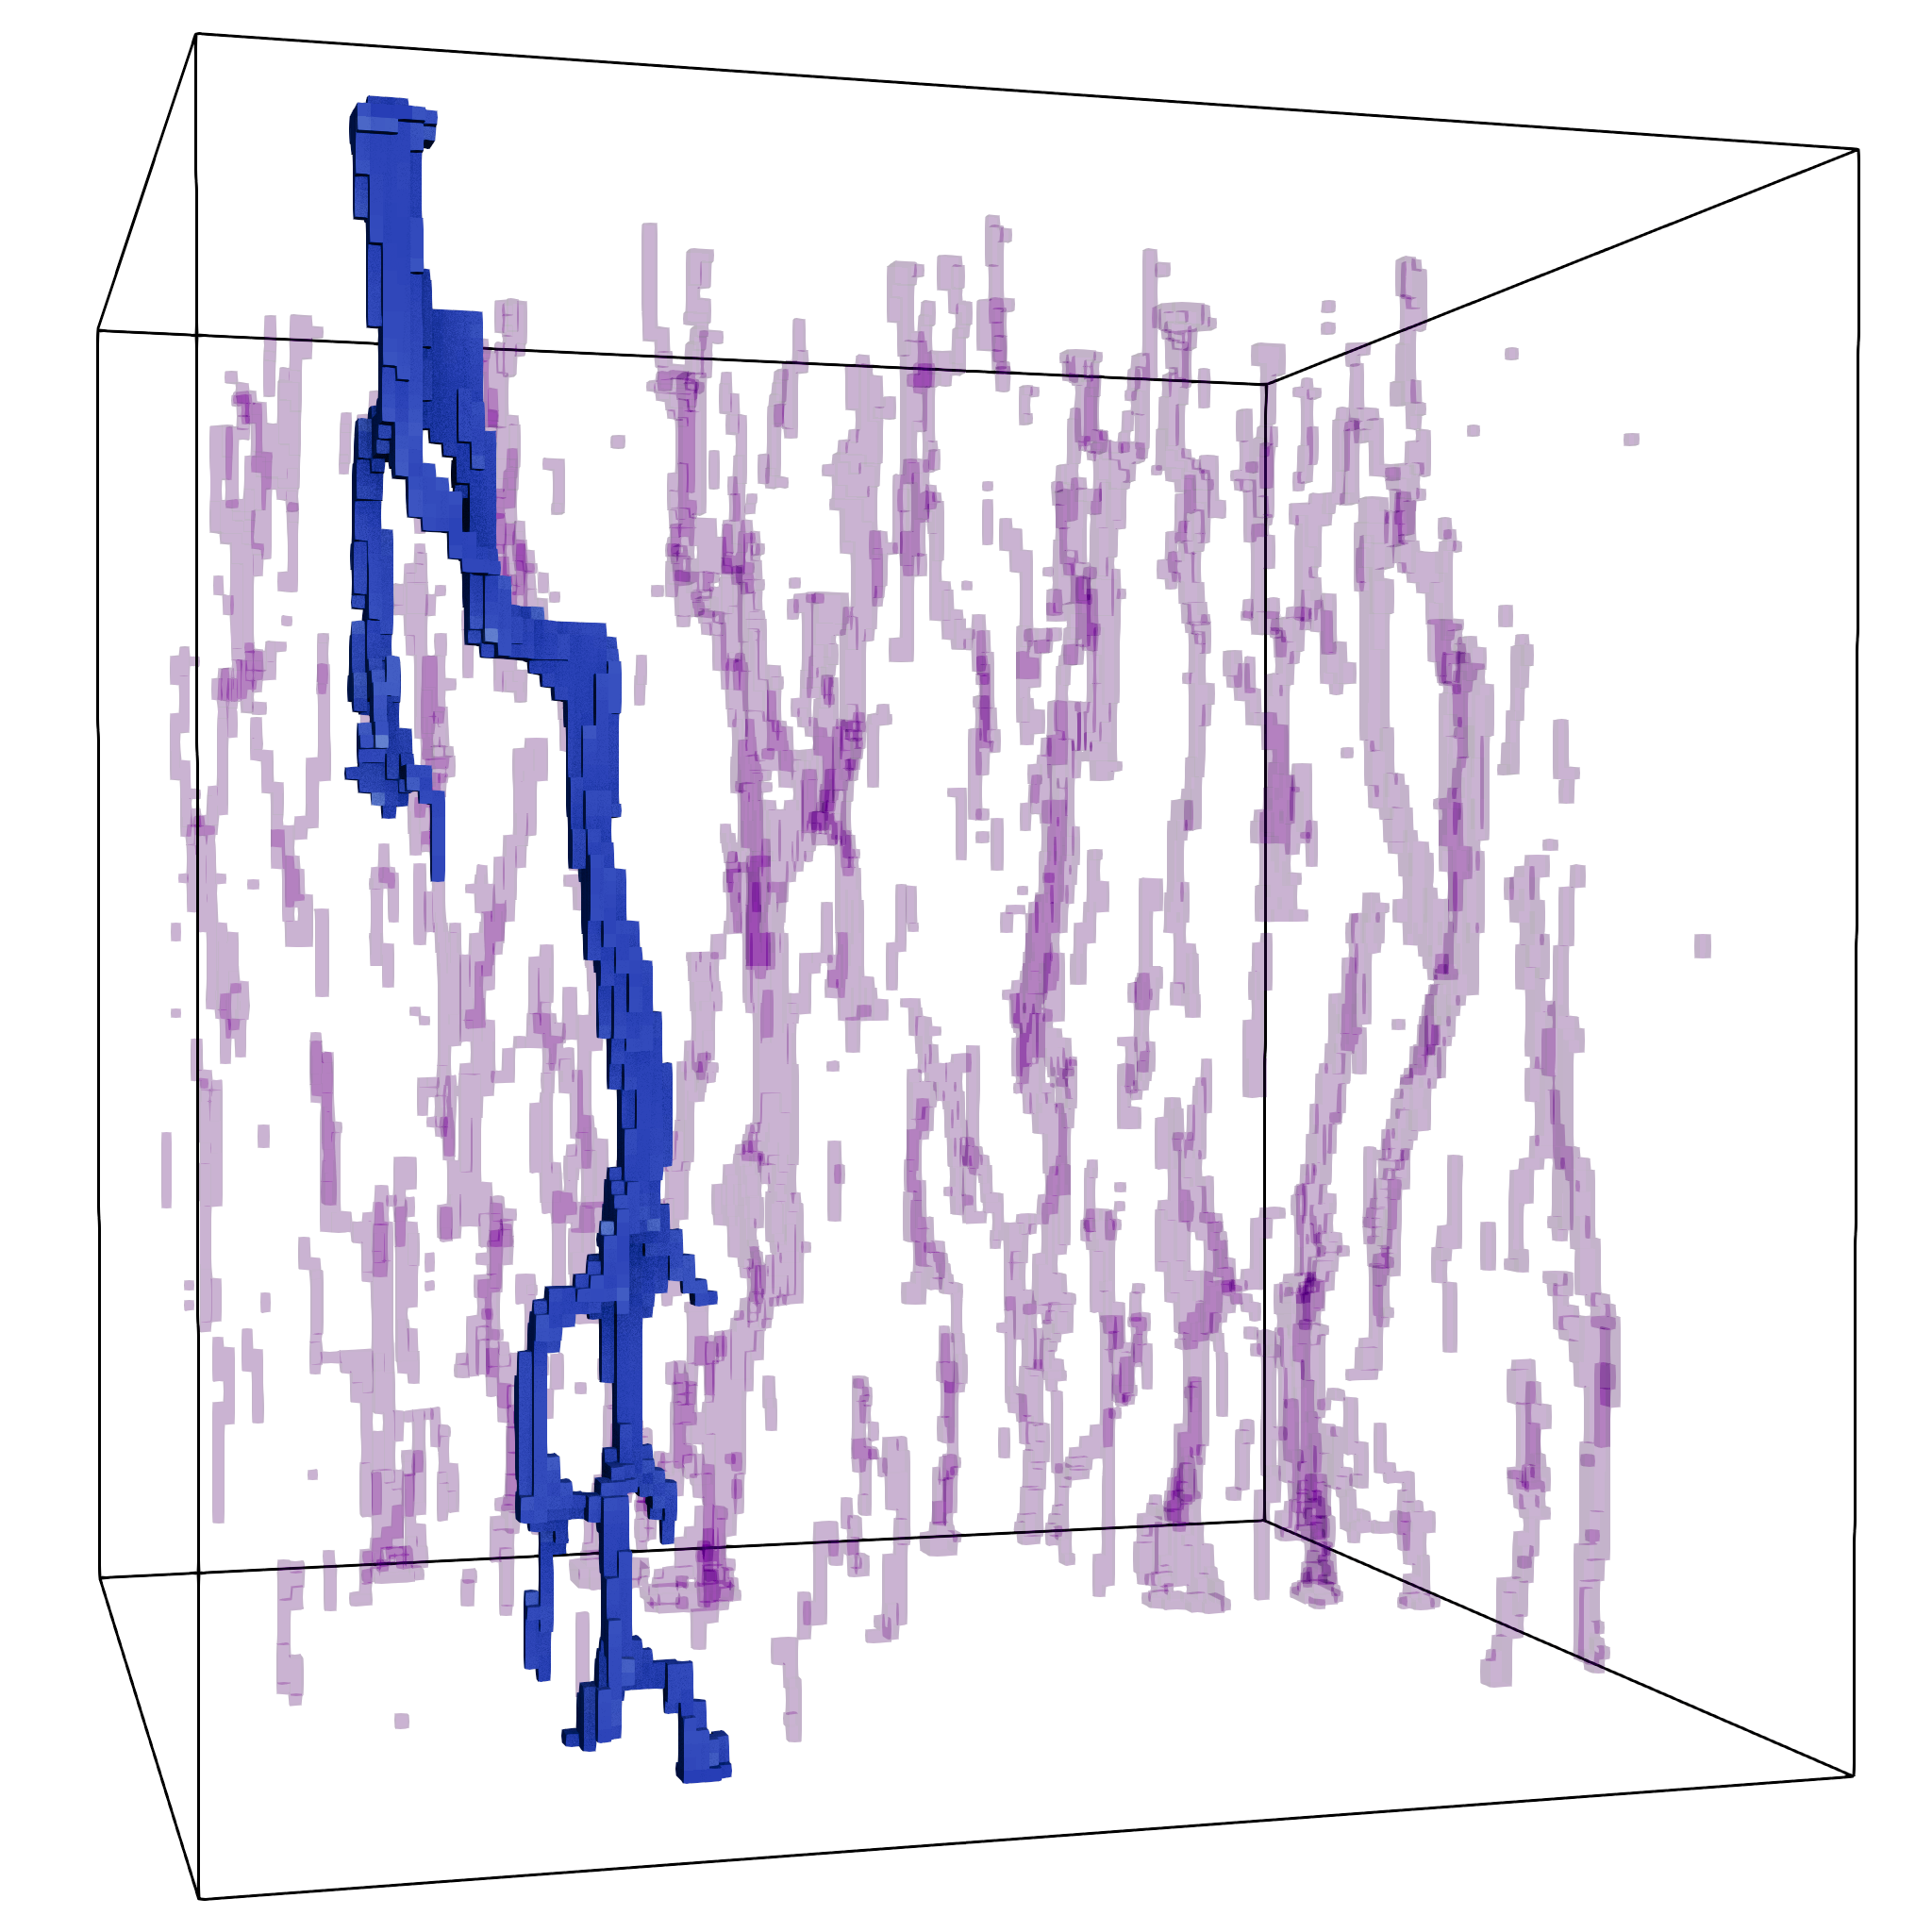
\includegraphics[width=0.333\textwidth]{figures/disturbance_result_3.png}}
\end{figure}
\vspace{-7mm}
\begin{minipage}[l]{0.93\textwidth}
\begin{align*}
	N_h &= 129 & T &\approx 1.7 \cdot 10^{-6} & \taumin &= 10^{-12} & 56 \text{ MPI-процессов} \\
	N_t &= 22000 & \Tol &= 10^{-2} & \taumax &= 10^{-7} &
\end{align*}
\end{minipage}
\end{frame}


\begin{frame}{Расчет №2: случайные возмущения}
\vspace{-4mm}
\begin{figure}
	\captionsetup[subfigure]{labelformat=empty}
	\subfloat[]{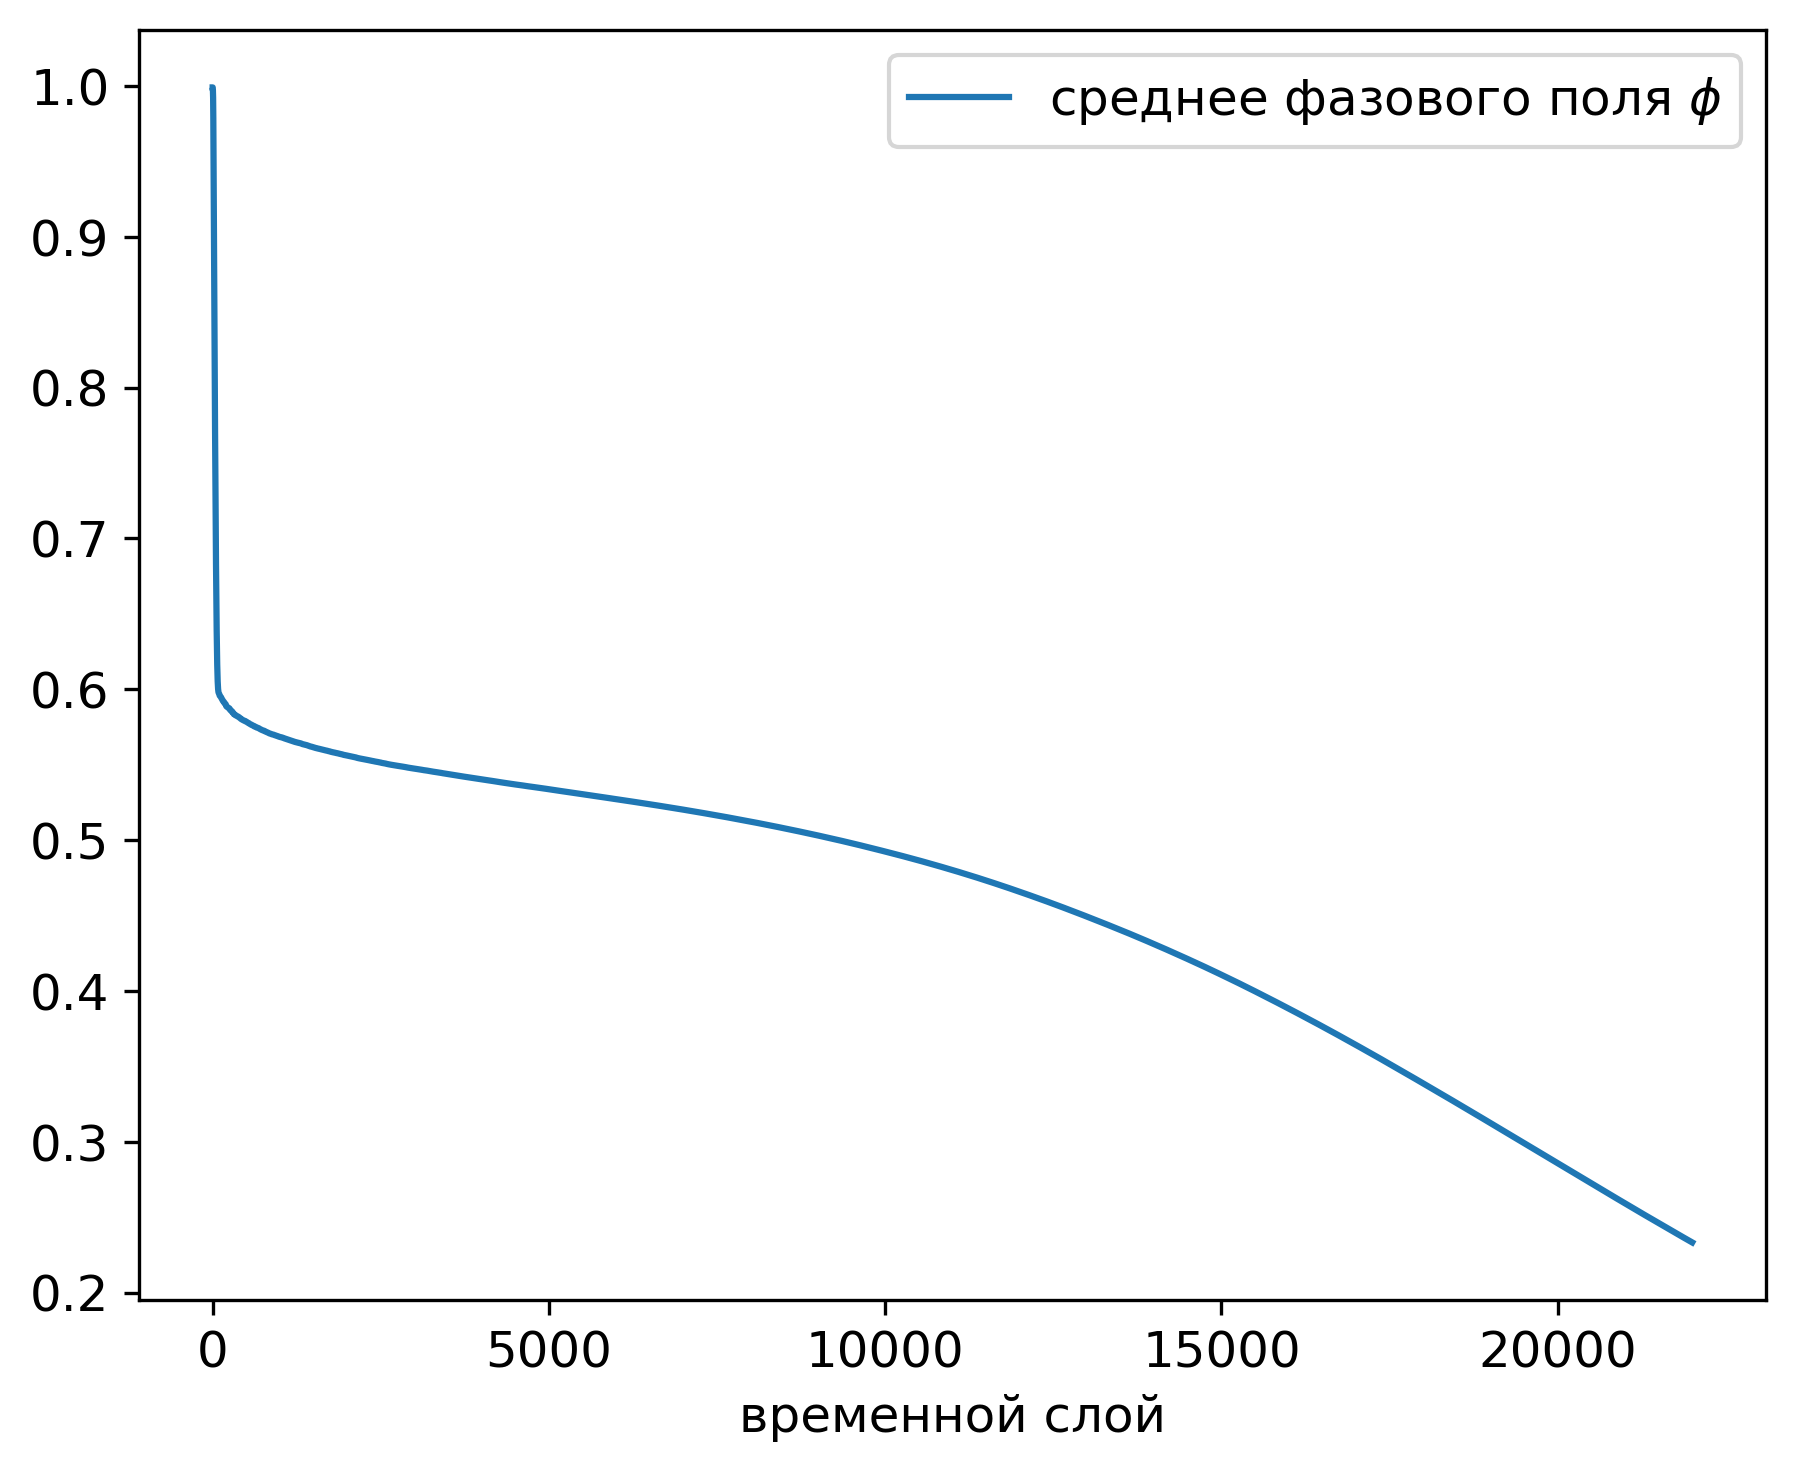
\includegraphics[width=0.49\textwidth]{figures/disturbance_phi_mean.png}}
	\hfill
	\subfloat[]{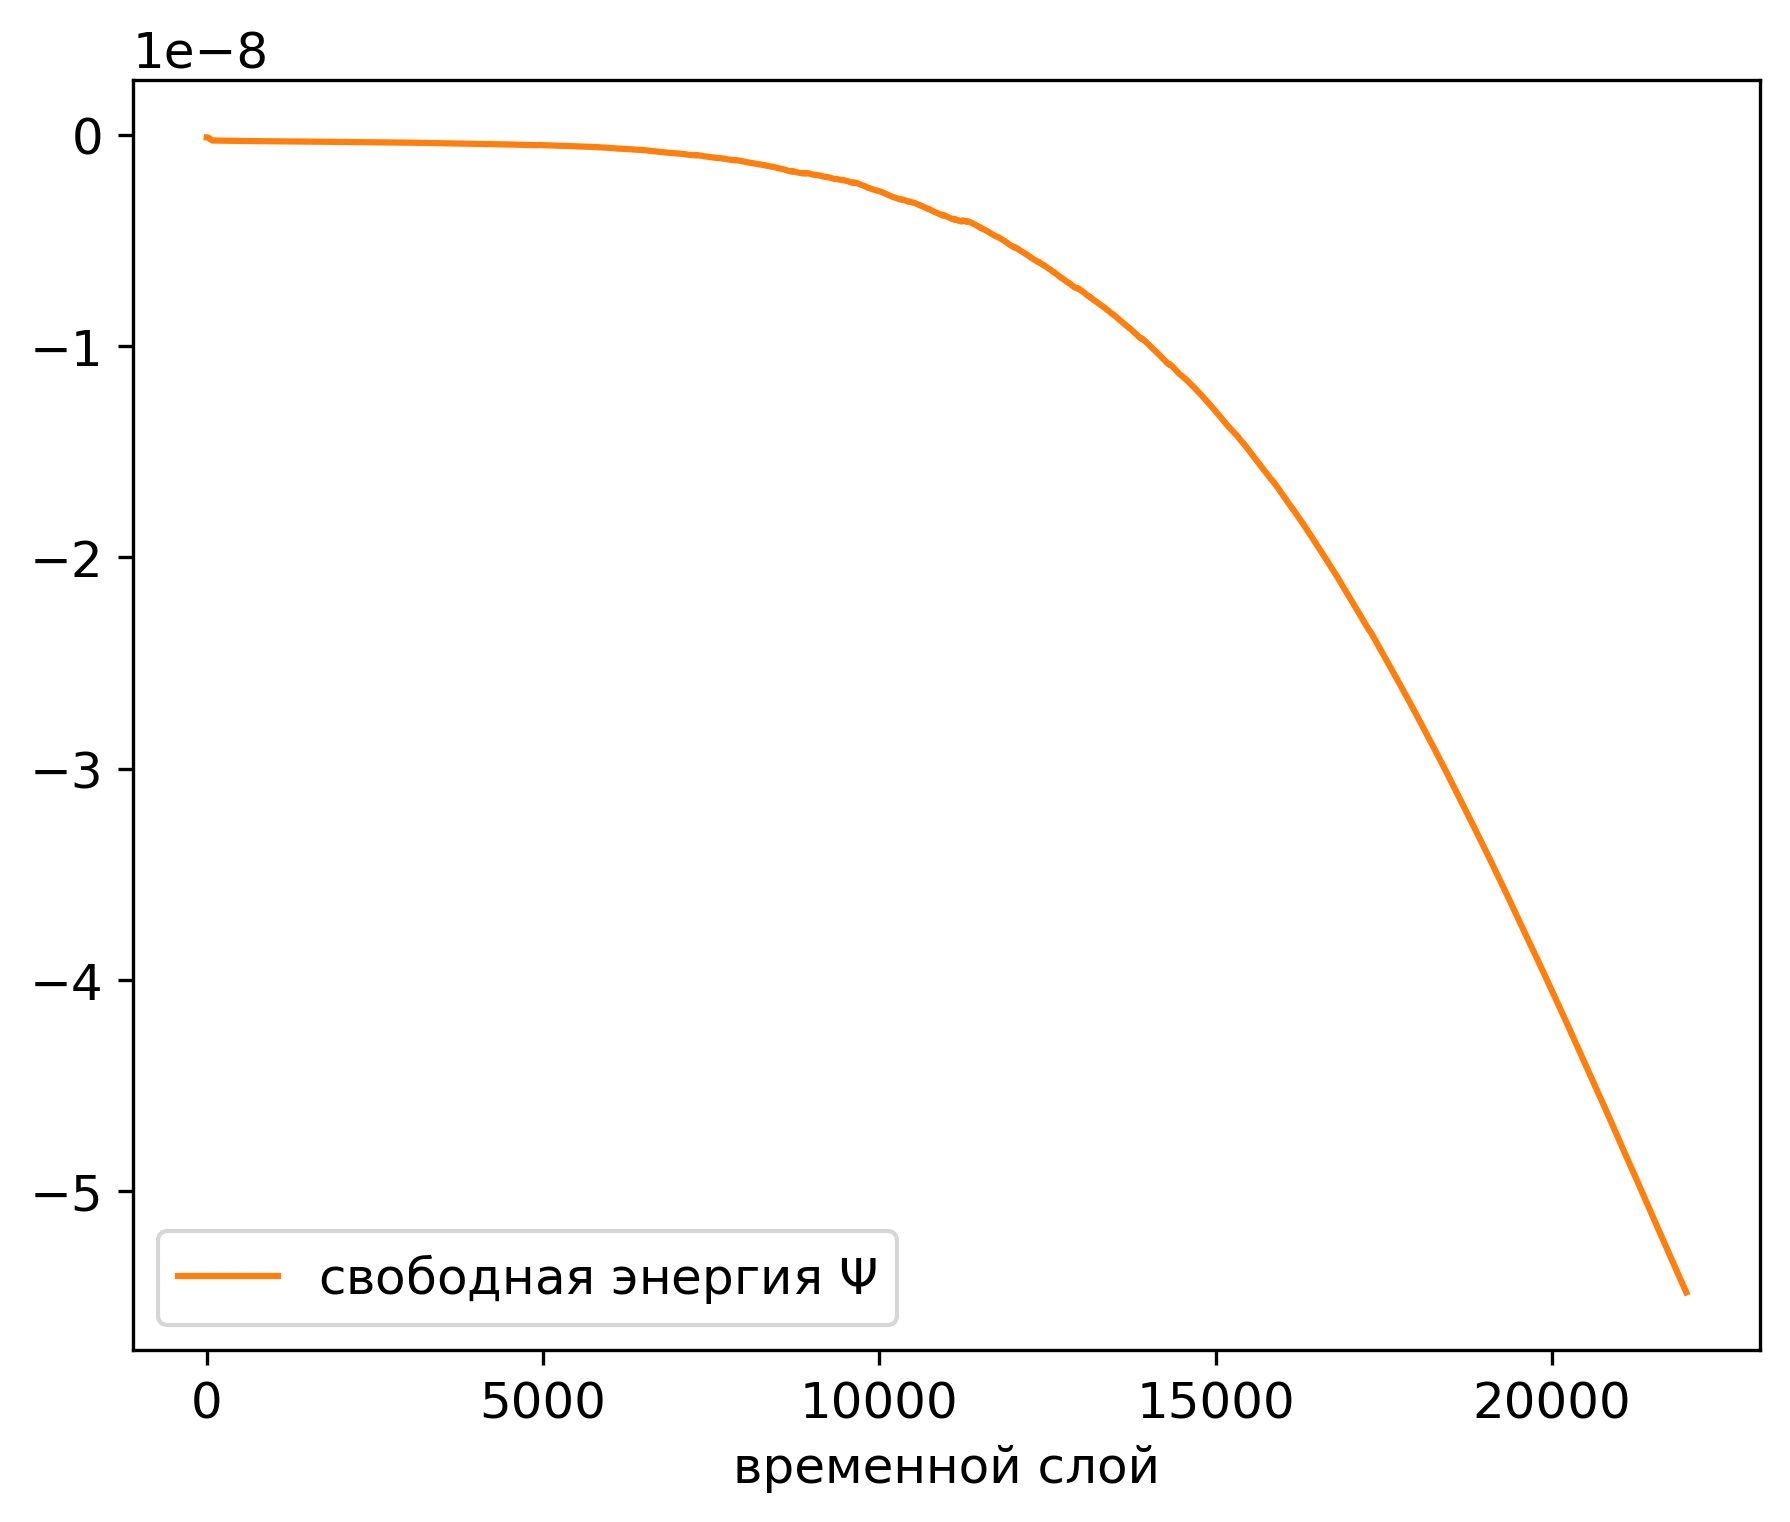
\includegraphics[width=0.49\textwidth]{figures/disturbance_energy.png}}
\end{figure}
\vspace{-13mm}
\begin{itemize}
    \item $\cfrac{d \Psi}{dt} = -\cfrac{1}{m} \, \intOmega (\partial \phi / \partial t)^2 d \vx \leqslant 0 \quad$ (выполнено)
\end{itemize}
\end{frame}


\begin{frame}{Сравнение эффективности расчетов}
\begin{center}
Время расчета (ч) в различных условиях \\[2mm]
\begin{tabular}{|%
	>{\centering\arraybackslash}m{5cm}|%
	>{\centering\arraybackslash}m{4cm}|%
	>{\centering\arraybackslash}m{4cm}|%
}
	\hline
	&& \\[-3mm]
	\multicolumn{1}{l}{Начальные условия}	&
	\multicolumn{1}{l}{С адаптацией}		&
	\multicolumn{1}{l}{Без адаптации}		\\[-2mm]
	&& \\[-1.5mm]
	\hline
	&& \\[-3mm]
	<<иголка>>				& $6.67$		& $105.12$	\\[1mm]
	&& \\[-3mm]
	случайные возмущения	& $5.09$		& $38.2$	\\[1mm]
	\hline
\end{tabular}
\end{center}
\vspace{2mm}
\parind Проверяется качественное совпадение процессов в системе
\end{frame}


\begin{frame}{Заключение}
\large
\begin{itemize}
	\item В упрощенной постановке задачи проверена работа трех методов \\ адаптации расчетного шага по времени
\end{itemize}
\vspace{1mm}
\begin{itemize}
	\item Наиболее эффективный (и наиболее простой) из методов внедрен \\ в ПО для моделирования
\end{itemize}
\vspace{1mm}
\begin{itemize}
	\item Получено значительное ускорение расчета в модельных постановках задачи
\end{itemize}
\end{frame}

{
\nologo
\begin{frame}{Литература}
\vspace{-2mm}
\printbibliography
\end{frame}
}

\begin{frame}{}
\begin{center}
	\LARGE
	Спасибо за внимание!
\end{center}
\end{frame}

\end{document}
